\documentclass{article}
\usepackage{appendix}
\usepackage{graphicx, float} % required for inserting images
\usepackage[utf8]{inputenc}
\usepackage{amsmath, amssymb, amsthm}
\usepackage{listings}
\lstset{breaklines=true}
\graphicspath{{\string~/Desktop/git/first-repo/wireless/report/snapshots}}
\usepackage[letterpaper, top=1in, bottom=1.1in, right=1in, left=1in]{geometry}
\renewcommand{\baselinestretch}{1.15} %line spacing
\usepackage{tocloft}
\usepackage{cite}

\title{7COM1076-0901-2024 - Wireless, Mobile and Multimedia Networking}
\author{22076082} 
\date{\today}

\begin{document}
\maketitle
\vspace{80pt}
\begin{center}
	\huge{Software Defined Networking(SDN) emulation with Mininet and OpenFlow} \\ [100pt]
	\vspace{80pt}
	\large{University of Hertfordshire} \\
	\large{Hatfield}
\end{center}

\newpage
\tableofcontents
\newpage
\listoftables
\listoffigures

\newpage
\begin{abstract}
The world has been considered a digital society with the intervention of the Internet. These computer networks form a strong foundation in the manner we access information, communicate, and handle data, providing convenience in various aspects of life. This technology relies strongly on the operations of traditional IP networks and despite being widely adopted, they do get complex and hard to manage in terms of configuration according to predefined policies and reconfiguration in response to load, faults, and changes. On top of that, conventional networks are vertically integrated(the control plane and data plane are bundled together). Emerging technologies such as Software-Defined Networking (SDN) provide a convenient approach in handling computer networks. SDN brings a proposed paradigm which changes state of affairs by separating the network's control logic from the data plane. This approach enables centralisation of network control and ability to program the network improving network availability, scalability, and management. This report presents a practical use-cases of SDN. It starts by utilising concepts of SDN in both a wireless and wired network scenario, an Ad-Hoc Network for emergency scenario, and multi-cast video streaming. We measure and test out performance metrics such as throughput and jitter for communications under Session Initiation Protocol (SIP) and UDP(connectionless) communication in client-server scenario. All activities are carried out on a single machine running Linux with underlying applications such as Mininet, Open Network Operating System(ONOS) and Wireshark.
\end{abstract}

\newpage
\section{Introduction}
Since the conception and realisation of the Advanced Research Projects Agency Networks(ARPANET)\cite{5432117}, developments and innovations in computer networks has seen a significant growth in size and requirements and navigating traditional network switches has become a challenge. In traditional networks, the control plane operation has a distributed infrastructure that requires protocols such as OSPF, STP, EIGRP, to operate independently on network devices. The forwarding decision which is the process of determining how to send a packet from one device (such as a router or switch) to another device within a network, based on certain criteria is performed by these network devices. This decision is made based on the information available in the routing table (for routers) or the switching table (MAC table) (for switches). It is accepted that the network devices connect but there is no centralised machine to manage or summarise the whole network\cite{Haji_Zeebaree_Saeed_Ameen_Shukur_Omar_Sadeeq_Ageed_Ibrahim_Yasin_2021}. Also, the distributed control and transport protocols running inside routers and switches makes it complex to express desired high-level network policies since network operators must configure each individual network device separately\cite{6994333}. This main issue is rectified by SDN, which introduces the needed network control, flexibility, and programmability that network operators want.\\
\subsection{Software-Defined Networking (SDN) and OpenFlow} 
Software-Defined Networking (SDN) is a computer technology that brings a change to the limitations of current computer networks infrastructure. SDN\cite{6587999} decouples the control and data plane of a network leaving the switch with the simple function of forwarding packets based on a set of rules. By doing so, it breaks the vertical integration of conventional networks as the control logic is separated from the data plane i.e. the underlying switches and routers that forward the traffic\cite{6994333}. To make possible the communication between the controller and the network devices, OpenFlow\cite{6587999} is used in conjunction with SDN. OpenFlow standardises the communication between the switches and the software-based controller in an SDN architecture. Researchers found it difficult to test out new ideas in current hardware because the source code of the software running on the network device cannot be modified making the infrastructure 'rigid'. As a result, a standardised protocol such as OpenFlow, to control flow table of switches through software was provided by identifying common features in the flow tables of the ethernet switches\cite{6587999}.\\The figures below show a comparison of the overview for traditional  and SDN network architecture.\\
	\begin{figure}[h]
        		\centering
		\small
        		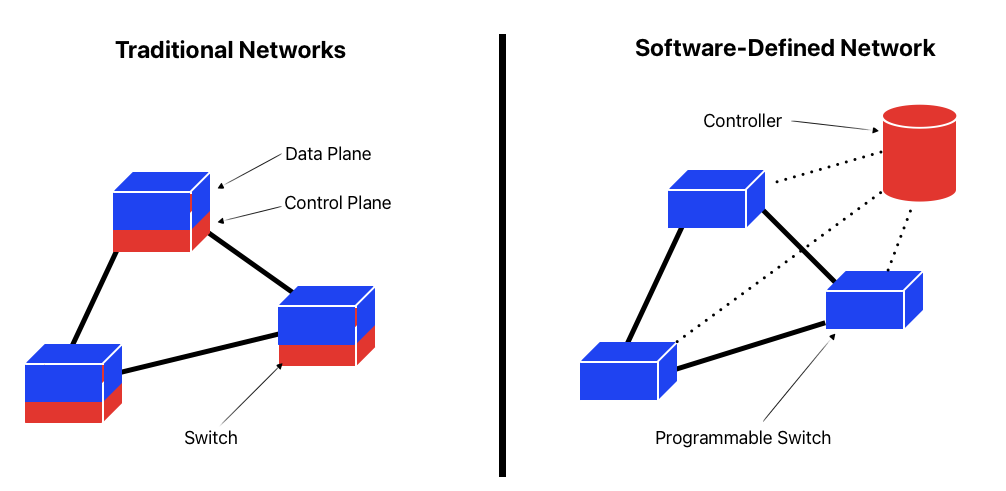
\includegraphics[width=0.7\linewidth]{SDN.png}
        		\caption{Architecture for Traditional and SDN networks}
        		\label{fig:SDN1}
	\end{figure}
    
	\newpage
    	\begin{figure}[h]
        		\centering
		\small
        		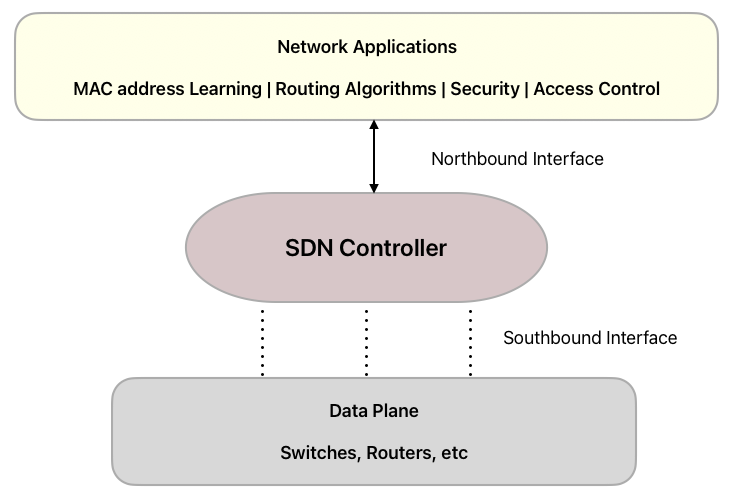
\includegraphics[width=0.5\linewidth]{SDN1.png}
        		\caption{SDN architecture}
       		 \label{fig:SDN2}
    	\end{figure} 
The underlying network applications or packages which are the softwares for the logical operations within the network are installed and activated on the SDN controller. These applications are known as the Northbound APIs or interface as shown in fig.2. The Southbound interface consist the protocols that facilitates communication between the remote SDN controller and the network devices, for example the OpenFlow\cite{10220519} protocol. Examples of such network applications can be STP, routing algorithms, and access control and examples of a SDN controller can be the ONOS controller. The prospect of such architecture is noticed in terms of ease of network management, programmability and openness to innovations and virtualisation it presents.
\subsection{Mininet}
For the scope of this paper, we aim to determine and investigate the convenience of SDN networks in a variety of network scenarios and requirements. To test out the efficiency, reliability, cost, and flexibility of the SDN approach in our network designs, the experiments are carried out on a network emulators known as Mininet. It is one of the many network simulation tools( another example is OMNETT++ ) that have been developed to virtualise and test network performance\cite{10220519, Haji_Zeebaree_Saeed_Ameen_Shukur_Omar_Sadeeq_Ageed_Ibrahim_Yasin_2021}. \\\\ Mininet\cite{6860404} provides a system that allows rapid prototyping of large networks and creates scalable software-defined networks using lightweight virtualisation mechanism. This alleviates the downside of conventional networking by providing a centralised view of the network and paves way for more controllability in managing the way networks should operate regardless of their size or their complexity. \\\\
Since research on this topic is still in progress, there are not many devices such as routers and switches that implement SDN functionalities, moreover, the existing ones are very expensive. Thus, in order to enable researchers to perform experiments and test novel features of this new paradigm in practice at a low financial cost, one solution is to use virtual network emulators such as Mininet. It creates SDN elements, customises them, and shares them among other networks and performs interactions\cite{6860404}.
\newpage
\subsection{Emulation environment specifications}
For this experiment, we utilise a microcomputer iMac with the following specifications: Processor 3 GHz 6-Core Intel Core i5, 16GB of ram, running the macOS 15.1, and VirtualBox Oracle VM version 7.1.2.
In this microcomputer, under the management of VirtualBox, we installed the following guest operating systems: Mininet emulator version 2.0 on Linux operating system Ubuntu 64bits with 4GB of RAM; ONOS controller version 4.2.14.
\section{Task 1 - WiFi Network Emulation}
In this task, we emulate a wireless network designed for a floor in the new building. For this purpose, we emulate 3 stations and 5 access points. The stations may represent a smart hand-held device which can vary from smartphone to a laptop, UE or to any WiFi compatible device. The stations carry a Class C private IP address of the same network. Access points are connected using a physical link facilitating a linear topology. The new building would create a minimalistic noise threshold of -91dBm. The access points are positioned strategically within the floor to make space for a signal dead-zone(red-spot) and 3 stations will be in mobility state to emulate real-life network scenario. \\ A python script will contain the code for this configuration and upon completion, we start the network using Mininet on a Linux terminal and view the network emulation on the Mininet-GUI feature while having to observe access point association, full connectivity between all nodes in the network on the Mininet CLI, and briefly understand how communication channels are used in a wireless network. \\\\
The figures below show the outline of the floor-plan in context and position of APs and  stations in the design.
    	\begin{figure}[h]
		\centering
        		\minipage{0.5\textwidth}
        		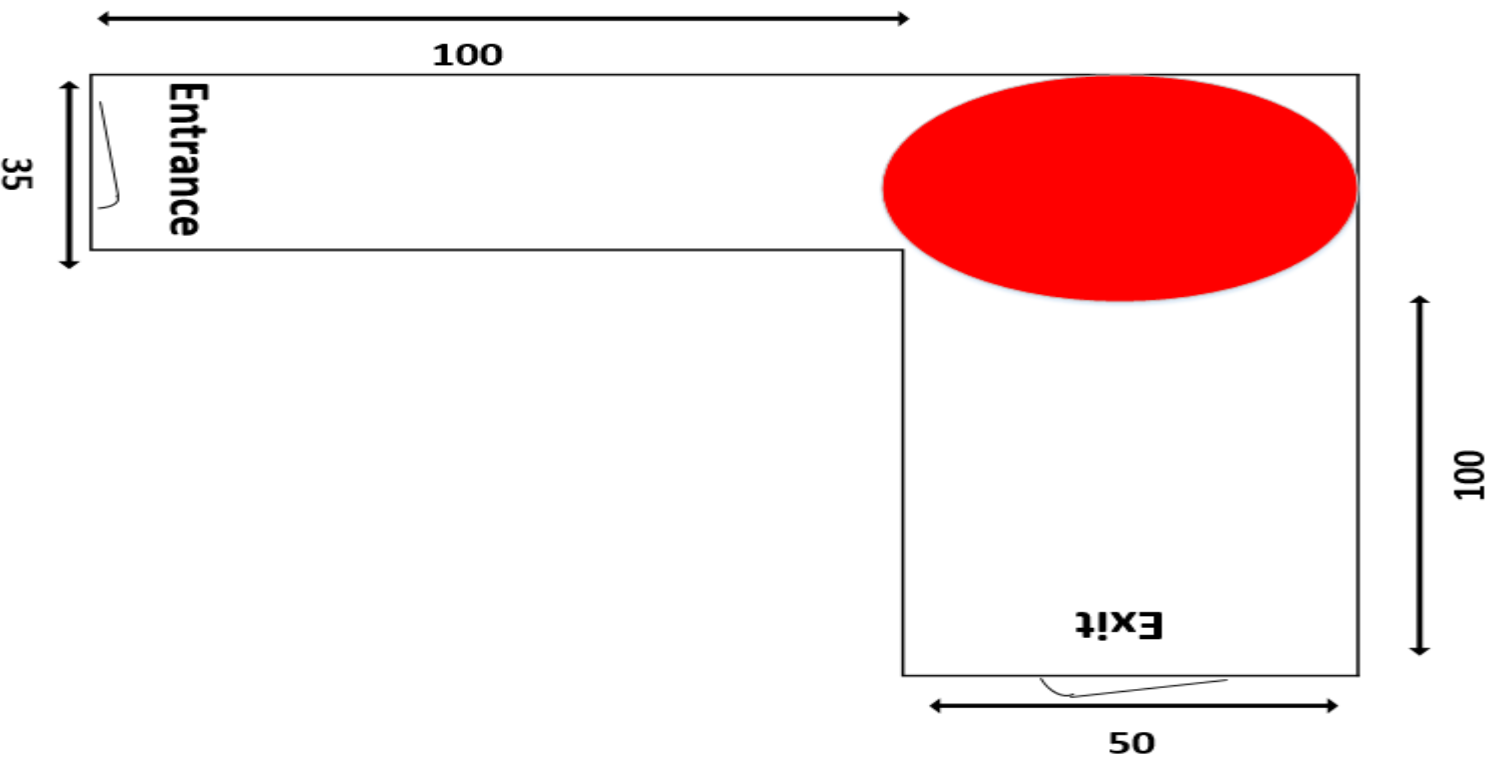
\includegraphics[width=0.9\linewidth]{floorplan1.png}
        		\caption{Floor-plan}
        		\label{fig:t1-1}
        		\endminipage
        		\minipage{0.4\textwidth}
        		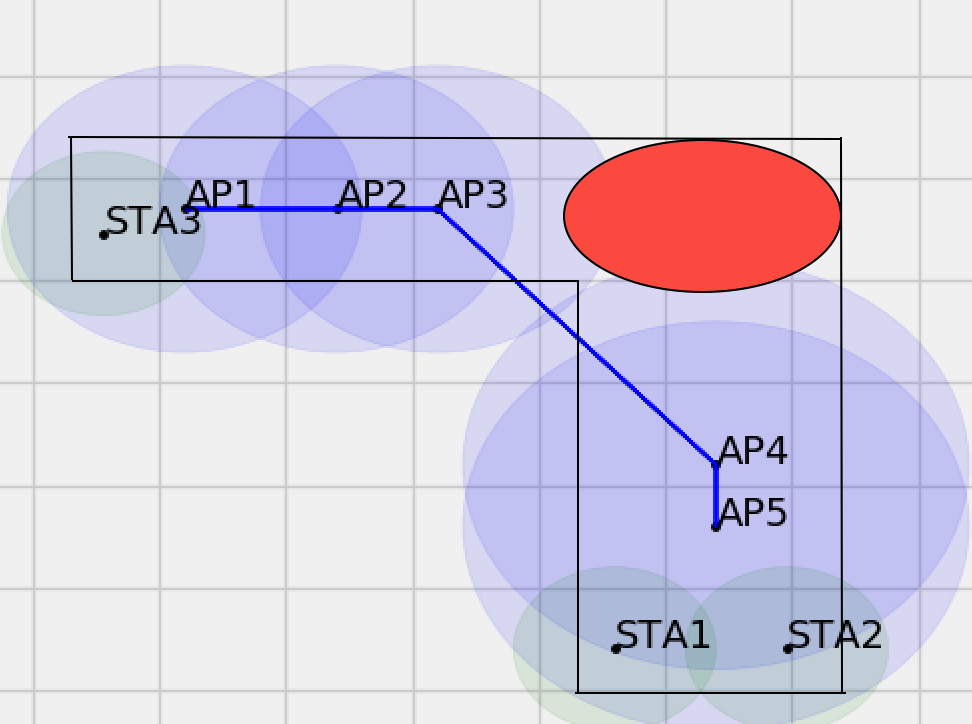
\includegraphics[width=0.9\linewidth]{floorplan.png}
        		\caption{Floor-plan with network topology}
       		\label{fig:t1-2}
       		\endminipage
    	\end{figure} 
\subsection{Design and Configuration}
Both figures show the outline of the floor-plan in context with the dimensions included on fig. 3 while fig. 4 is a snapshot of the Mininet GUI with the positions of the stations and access points and the range of coverage of all devices. The 'red-spotted' zone as seen remains free of WiFi signals as required in the design. \\ Table 1 contains the details of stations and access points which are used for the network configuration in a python script. All three stations share the same network address and have full authenticated access to each access points. \\ The access points are positioned strategically and linked serially to ensure the required zones within the floor have strong WiFi frequency coverage and support full connectivity of the stations. To emulate real networking scenario, mobility is included for the stations, details are shown in Table 2. Mobility attributes in terms of velocity or speed of motion for each station are specified. The mobility attributes are added to the python code for the network configuration which is captured in the appendix section of this document.
  	\begin{table}[h]
        		\begin{tabular}{|c|c|c|c|c|c|c|c|}
        			\hline
        			DEVICE & MAC & IPv4 & (x,y) & SSID & PASSWORD & RANGE & CHANNEL\\
        			\hline
        			STA1 & 00:00:00:00:00:10 & 192.168.50.11/24 & 15,115 & n/a & n/a & 20 & n/a \\
        			STA2 & 00:00:00:00:00:11 & 192.168.50.12/24 & 20,130 & n/a & n/a & 20 & n/a \\
       			STA3 & 00:00:00:00:00:12 & 192.168.50.13/24 & 140,10 & n/a & n/a & 20 & n/a \\
        			AP1 & 00:00:00:00:00:00 & n/a & 30,117.5 & AP1 & n/a & 35 & 1 \\
        			AP2 & 00:00:00:00:00:01 & n/a & 60,117.5 & AP2 & n/a & 35 & 1 \\
        			AP3 & 00:00:00:00:00:02 & n/a & 80,117.5 & AP3 & n/a & 35 & 1 \\
        			AP4 & 00:00:00:00:00:03 & n/a & 135,55 & AP4 & n/a & 50 & 1 \\
        			AP5 & 00:00:00:00:00:04 & n/a & 135,40 & AP5 & n/a & 50 & 1 \\
        			\hline
        		\end{tabular}
        \caption{Details of stations and access points}
        \label{tab:1}
    	\end{table}
    	\begin{table}[h]
       		\begin{tabular}{|c|c|c|c|c|}
        			\hline
        			DEVICE & START LOCATION & END LOCATION & START-STOP TIME & MOVING SPEED(min-max)  \\
        			\hline
        			STA1 & 15,115 & 115,10 & 10s-20s & min\_v=1, max\_v=5 \\
        			STA2 & 20,130 & 150,10 & 30s-60s & min\_v=5, max\_v=10 \\
        			STA3 & 140,10 & 15,120 & 25s-60s & min\_v=2, max\_v=7 \\
        			\hline
        		\end{tabular}
        \caption{Mobility of the stations}
        \label{tab:2}
    	\end{table}
\subsection{Results and Analysis}
Commencing the test, we prepare the python script for the network topology with all necessary libraries then run it with Mininet on the Linux terminal. The command \texttt{sudo ./<pycode filename>} is used to start the network using the configuration from the python script on Mininet. Mininet creates the SDN elements such as the controller, stations, and access points and sets up the topology as described in the python script. \\\\ The controller used in this task is a default one used by Mininet since it has not been specified. The access points are started and operated based on instructions from the controller. Fig. 5 \& 6 show the Mininet GUI view of the topology prior mobility and after mobility respectively. All stations are within strong WiFi signal coverage and successfully communicate with each other as shown in Fig. 8. \\\\ The \texttt{ping -c 3} command was utilised to send out 3 Internet Control Message Protocol(ICMP)\cite{1010101} packets between specified stations to determine full connectivity within the network. This uses a series of request \& reply messages to establish communication between stations. The results show all 3 packets were transmitted and received successfully, no packet loss, and took an average time of 2000 milliseconds for all communications which verifies the optimal performance of the network. \\\\ Prior mobility, we see that stations 1 \& 2 would likely be associated with AP1 and station 3 with AP5 due to their close proximity to these APs but when in mobility state, the stations will lose association with access points, go through a handoff operation, and get associated with the access point in close proximity at the end of mobility state. To confirm this, we use the \texttt{<station name> iwconfig} command on the Mininet CLI to pull the wireless interface information for each station as illustrated in Fig. 7. This same activity could be carried out on each station directly when accessed with the \texttt{xterm <station name>} command on Mininet CLI. \\\\ Briefly, wireless communication is based on digital signals that are transmitted from one end and received at another end over the radio frequency spectrum. Medium Access Control(MAC)\cite{1010101} is a mechanism devised to management how these radio channels are accessed by wireless capable devices for a wireless communication and have two main techniques; Contention-based \& Contention-free MAC. \\\\ At the end of this experiment, we experience the sort of flexibility SDN brings into wireless network configuration and management, cost of deployment,  quick response time, and overall summary of the network compared to the conventional methods of networking.
    	\begin{figure}[h]
        		\minipage{0.5\textwidth}
        			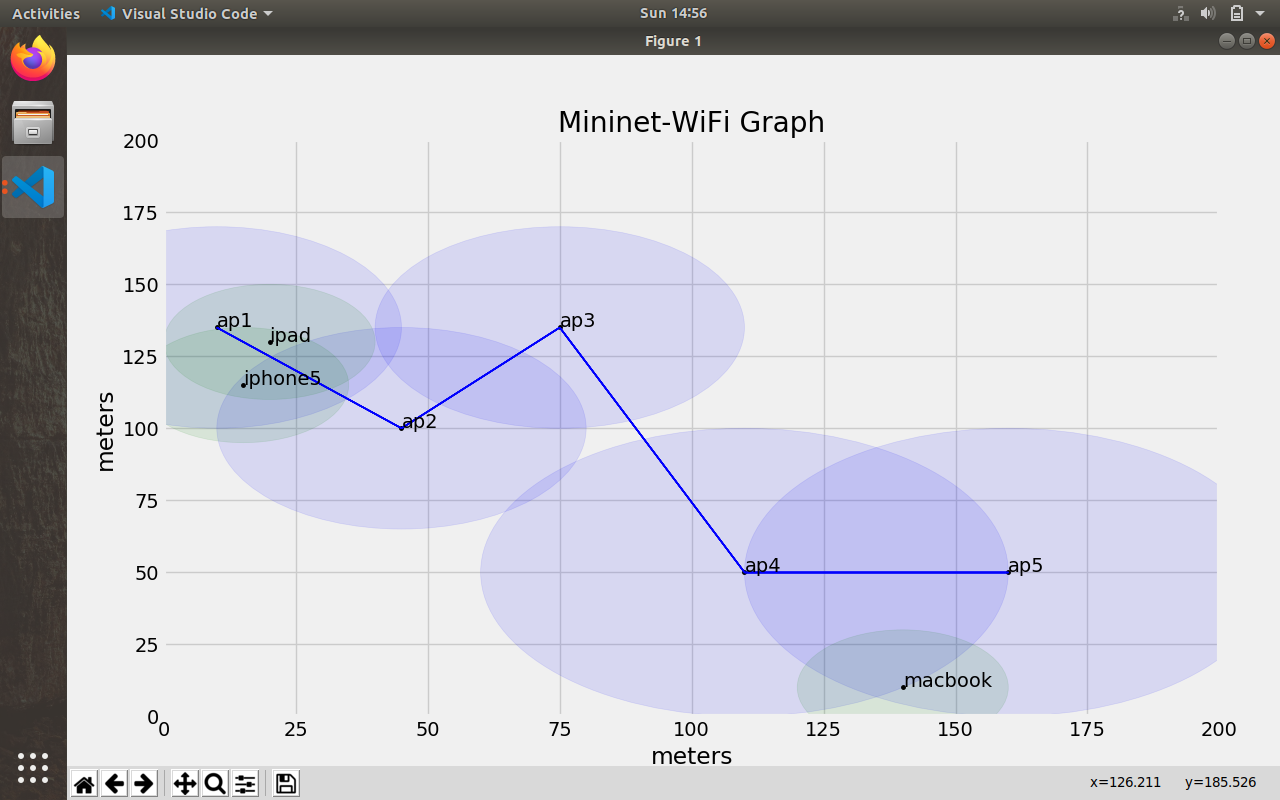
\includegraphics[width=0.9\linewidth]{beforeMobility.png}
        			\caption{Prior mobility}
       			\label{fig:t1-3}
        		\endminipage
       		\minipage{0.5\textwidth}
		\centering
        			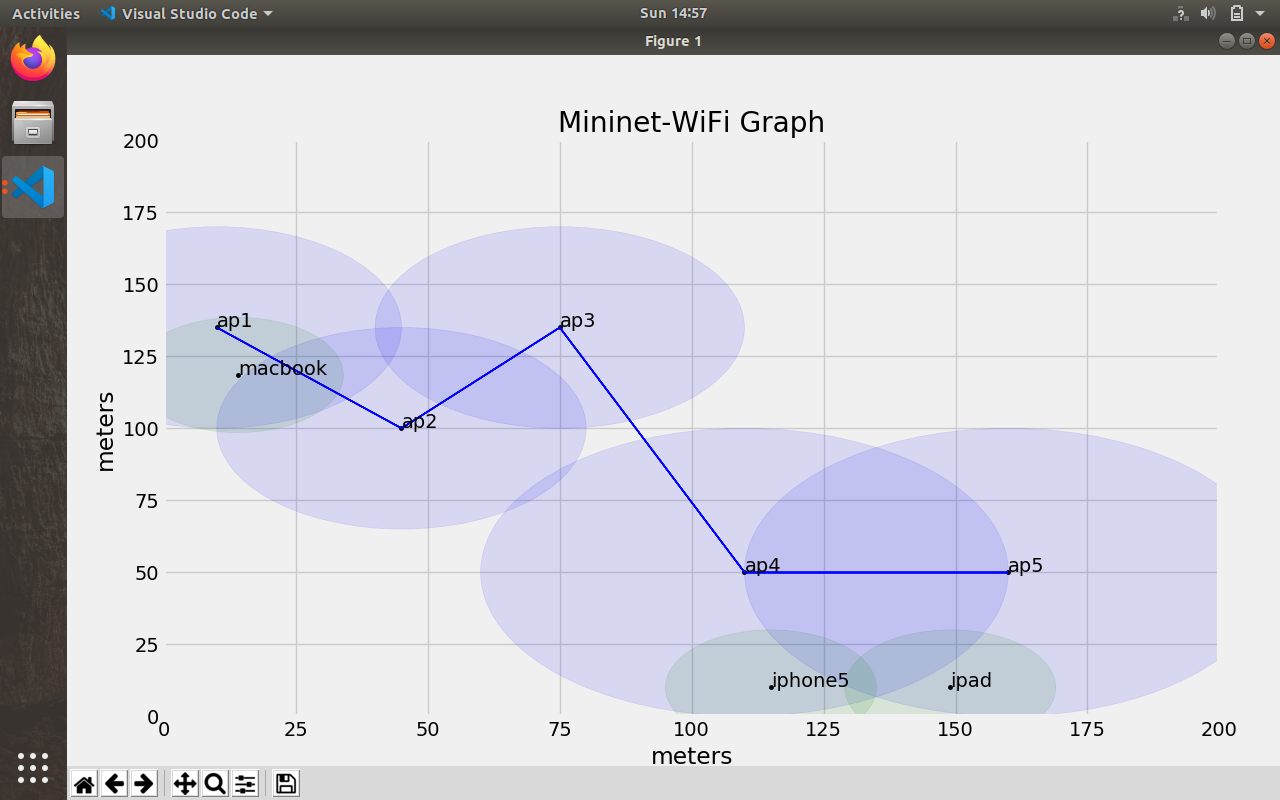
\includegraphics[width=0.9\linewidth]{afterMobility.png}
        			\caption{After mobility}
        			\label{fig:t1-4}
        		\endminipage\vspace{10pt}
        		\minipage{0.5\textwidth}
        			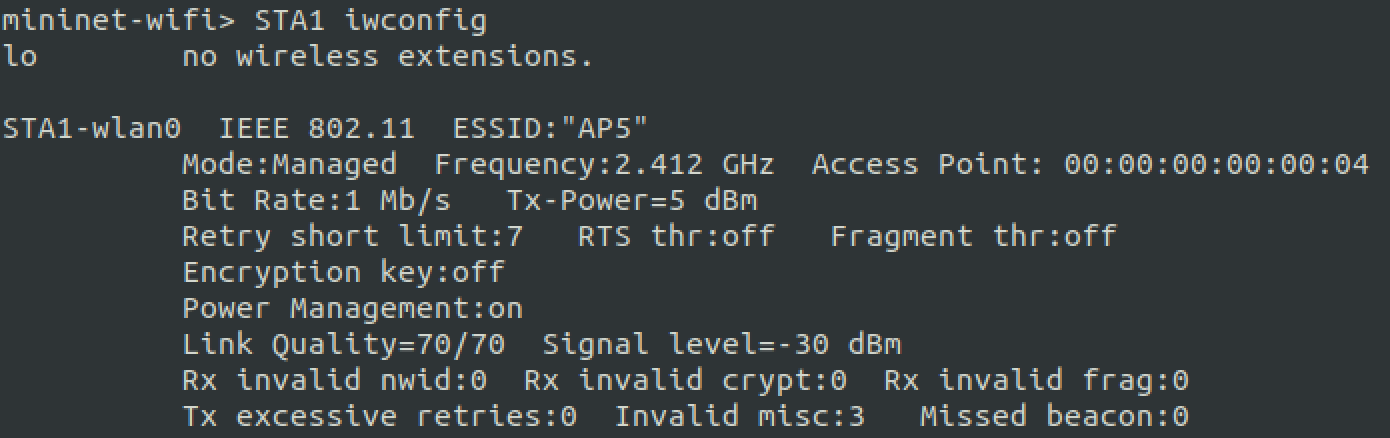
\includegraphics[width=0.9\linewidth]{sta1.png}
        			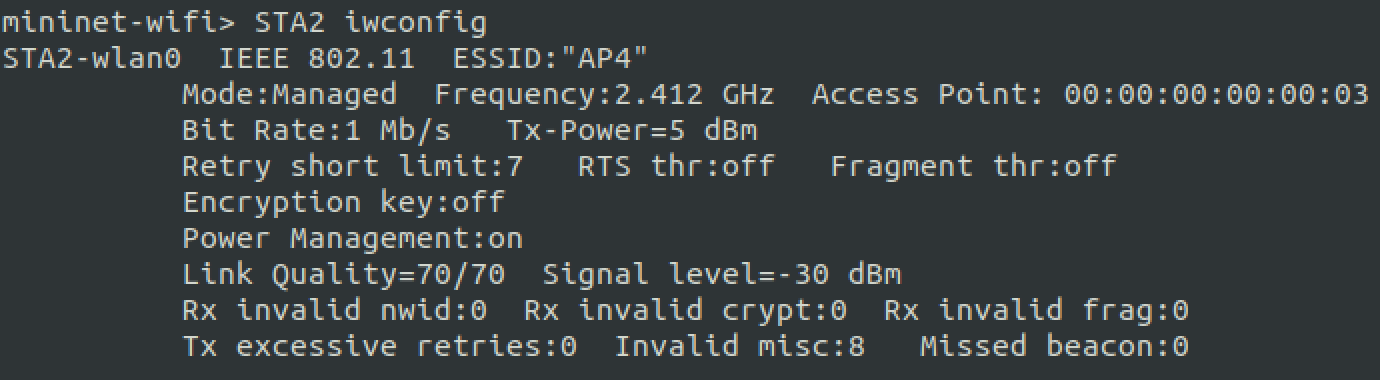
\includegraphics[width=0.9\linewidth]{sta2.png}
        			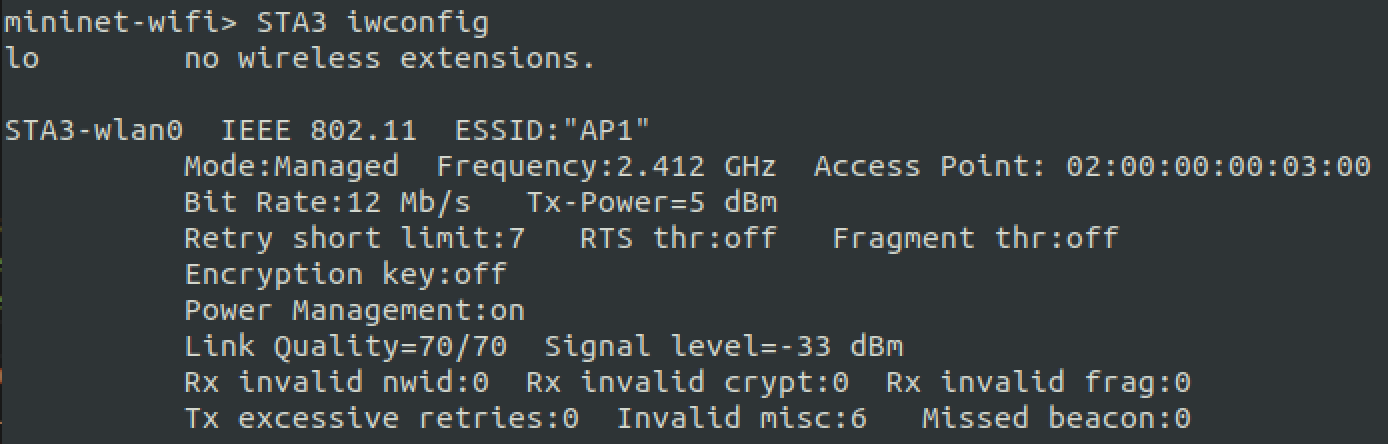
\includegraphics[width=0.9\linewidth]{sta3.png}
        			\caption{Access points connected after mobility}
        			\label{fig:t1-5}
        		\endminipage\vspace{10pt}
        		\minipage{0.5\textwidth}
        			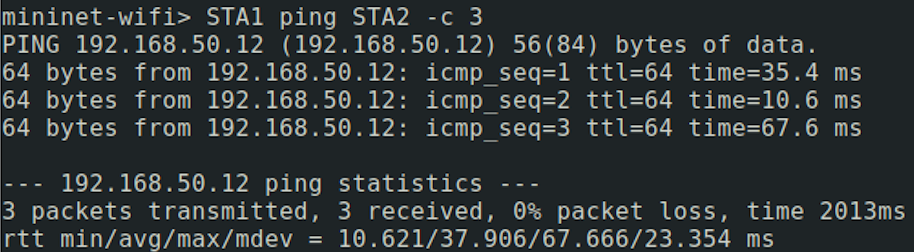
\includegraphics[width=0.9\linewidth]{ping1.png}
        			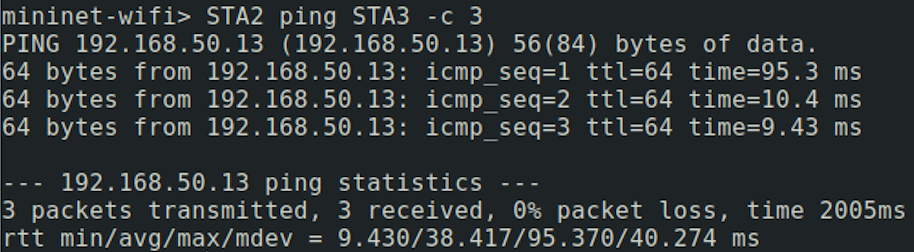
\includegraphics[width=0.9\linewidth]{ping2.png}
       			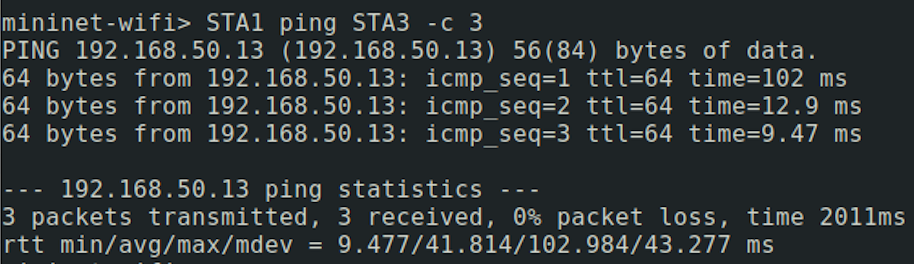
\includegraphics[width=0.9\linewidth]{ping3.png}
        			\caption{Full node connectivity}
        			\label{fig:t1-6}
        		\endminipage
    	\end{figure}

\newpage
\section{Task 2 - Adhoc Network Simulation}
In this task, we emulate an AdHoc network scenario at an emergency gathering car park at the new building when response units will communicate via AdHoc services. We evaluate some adhoc protocols to find which is best for the given situation. For this purpose, 3 stations are emulated and the adhoc protocols which will be tested are the 'batmand', 'batman\_adv', and 'olsrd' protocols. ICMP streams are initiated between the stations closest to each other and 3 VoIP for each adhoc protocol tested. For analysis of connection and network performance, we use a network protocol analytic tool known as Wireshark to inspect and capture traffic of a network in real-time. It shows details about protocols and can be used to generate a graphical or visualised view of network traffic.
\subsection{AdHoc Networks}
AdHoc\cite{1010101} networks are quick to deploy and dynamic form of networks that can be designed for a particular use-case. It is a wireless network however individual nodes can act as hops for forwarding packets and can move randomly within the local network. AdHoc networks are less reliant on infrastructure and efficient in setting up wireless communications in cases of emergencies or quick deployment.
    	\begin{figure}[h]
        		\centering
        		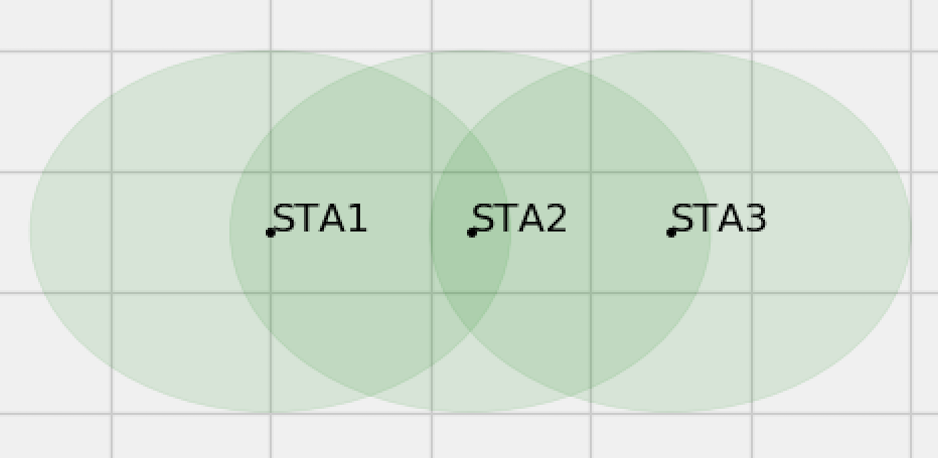
\includegraphics[width=0.4\linewidth]{adhoc.png}
        		\caption{Adhoc network with 3 stations}
        		\label{fig:t2-1}
    	\end{figure}
\subsection{Design and Configuration}
A python script is used for the configuration of the network where all 3 stations are created and configured with a protocol to support communication over the AdHoc network. Fig. 9 depicts the floor plan of the new building and emergency gathering car park with 3 stations in close proximity. Table 3 contains the station names, IPv6 and MAC addresses, their positions, range of radio frequency coverage, and wireless configuration with details about those fields below; 
	\begin{itemize}
		\item A\_HEIGHT: the height of the antenna typically in physical distance(metres) between the antenna and the ground or reference point
		\item A\_GAIN: the measure of how good an antenna converts input power into radio waves in a specific direction. Usually expressed in decibels (dB)
		\item SSID: Service Set Identifier, unique name used to identify a wireless local area network(WLAN)
		\item HT\_CAP.: High Throughput Capability, relates to 802.11n/ac standards to support high data rate and better performance 
	\end{itemize}
    	\begin{table}[h]
		\small
        		\begin{tabular}{|c|c|c|c|c|c|c|c|c|}
        			\hline
        			NAME & IPv6 & MAC & POSITION & RANGE & A\_HEIGHT & A\_GAIN & SSID & HT\_CAP\\
        			\hline
        			STA1 & 2024::11 & 00:00:00:00:01:11 & 20,10,0 & 30 & 1 & 5 & adhocUH & HT40+ \\
        			STA2 & 2024::12 & 00:00:00:00:01:12 & 45,10,0 & 30 & 2 & 6 & adhocUH & HT40+ \\
        			STA3 & 2024::13 & 00:00:00:00:01:13 & 70,10,0 & 30 & 3 & 7 & adhocUH & HT40+ \\
        			\hline
        		\end{tabular}
       	 	\caption{Adhoc stations configuration details}
        		\label{tab:3}
    	\end{table}
\newpage
\subsection{Results and Analysis}
After completion of the script, the network is started on the Linux terminal with the \texttt{sudo ./<python filename>} command. For this experiment, we aim to establish a successful connection between the closest stations in our setup i.e. between STA1 and STA2 and test out a VoIP connection between the stations under three different adhoc protocols. \\ The Session Initiation Protocol(SIP) which is a protocol used to establish, modify, and terminate multimedia sessions over IP networks will be initiated on one station as a server and on the other as client. The SIP commands are run on each stations directly accessing them with \texttt{xterm <station name>} on Mininet CLI. 
	\begin{itemize}
		\item on server(STA1): \texttt{sipp -sn -uas}
		\item on client(STA2): \texttt{sipp -sn uac <STA1 IPv4> -timeout 120}
	\end{itemize}
	\begin{figure}[h]
        		\centering
        		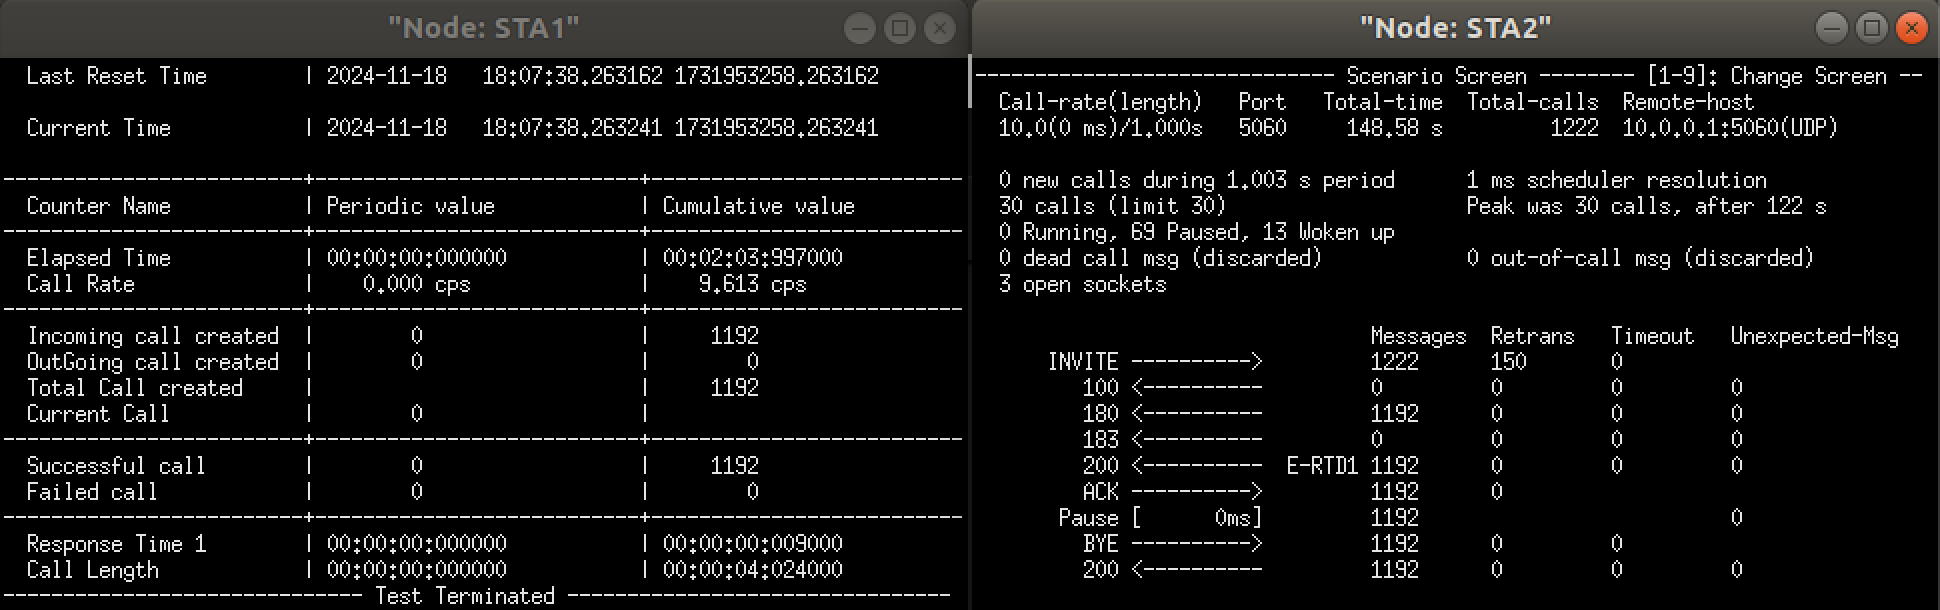
\includegraphics[width=0.6\textwidth]{batman_adv1.png}
        		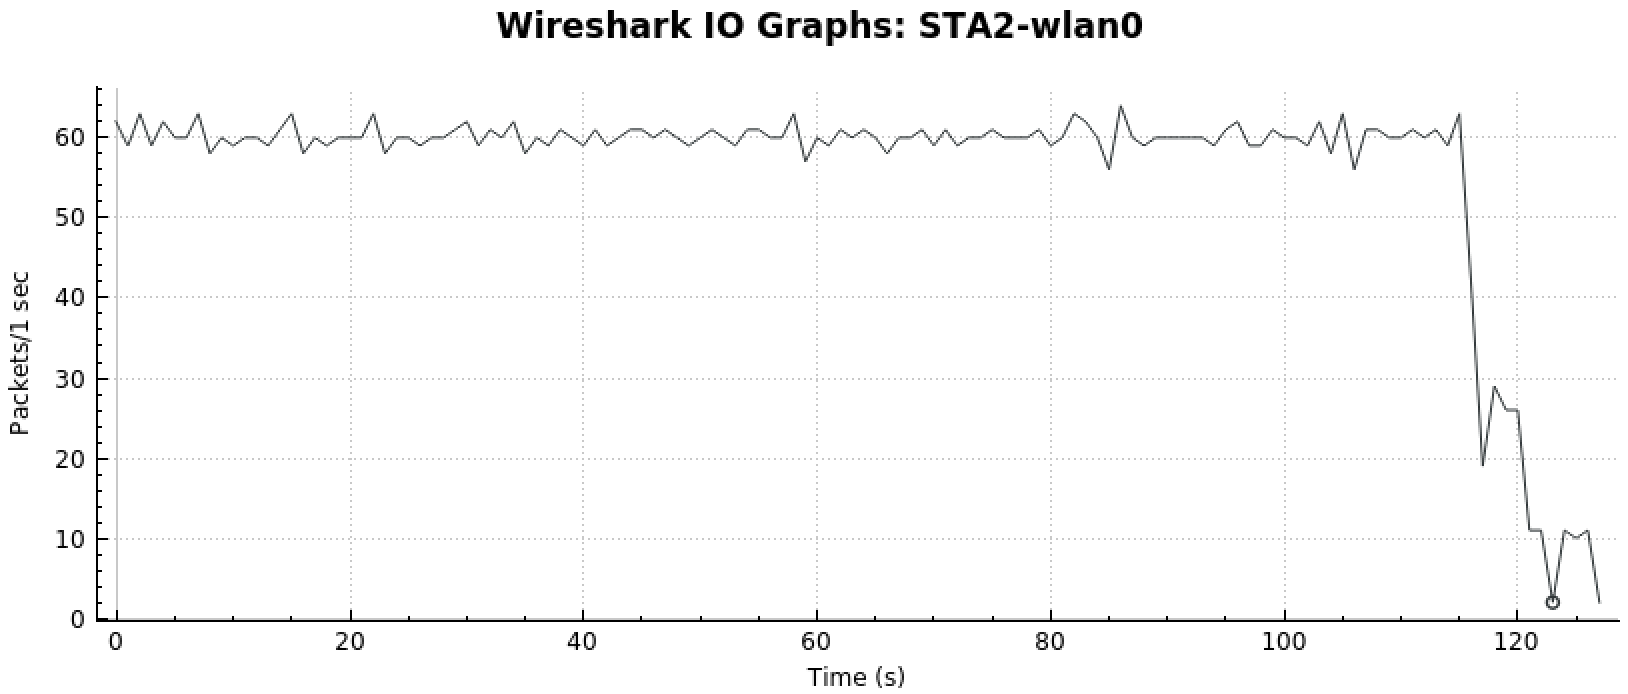
\includegraphics[width=0.6\textwidth]{batman_adv.png}		
        		\caption{SIP connection \& throughput under BATMAN\_ADV protocol}
        		\label{fig:t2-2}
    	\end{figure}
The \texttt{sipp -sn -uas} command sets up a User Agent Server on STA1 to respond to incoming SIP requests such as an INVITE messages with appropriate SIP responses such as 180 RINGING, 200 OK. \\ The \texttt{sipp -sn uac <STA1 IPv4> -timeout 120} command sets up STA2 as a User Agent Client to send INVITE messages to initiate SIP calls and wait for response  such as 180 RINGING and 200 OK. \\\\ We capture and inspect the communication on Wireshark by running another instance of xterm on the client station on the Mininet CLI, then entered the command \texttt{sudo wireshark} to launch Wireshark. After it launches, the interface for the client station is selected to view the detailed packet information and throughput graph is generated by clicking on the 'Statistics' tab in Wireshark then selecting 'I/O Graph' from the dropdown list.
    	\begin{figure}[h]
        		\centering
        		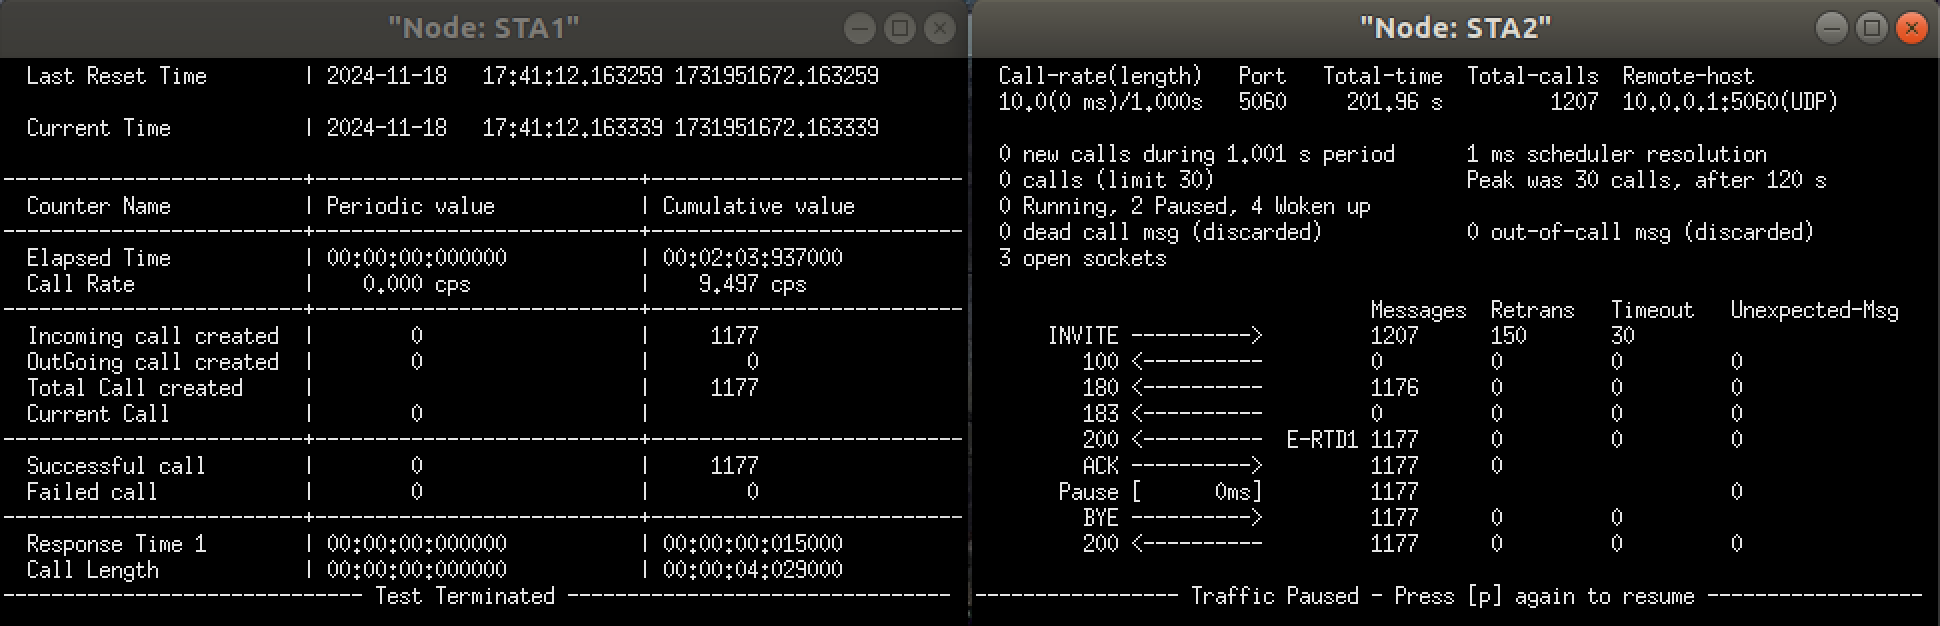
\includegraphics[width=0.6\linewidth]{batmand1.png}
		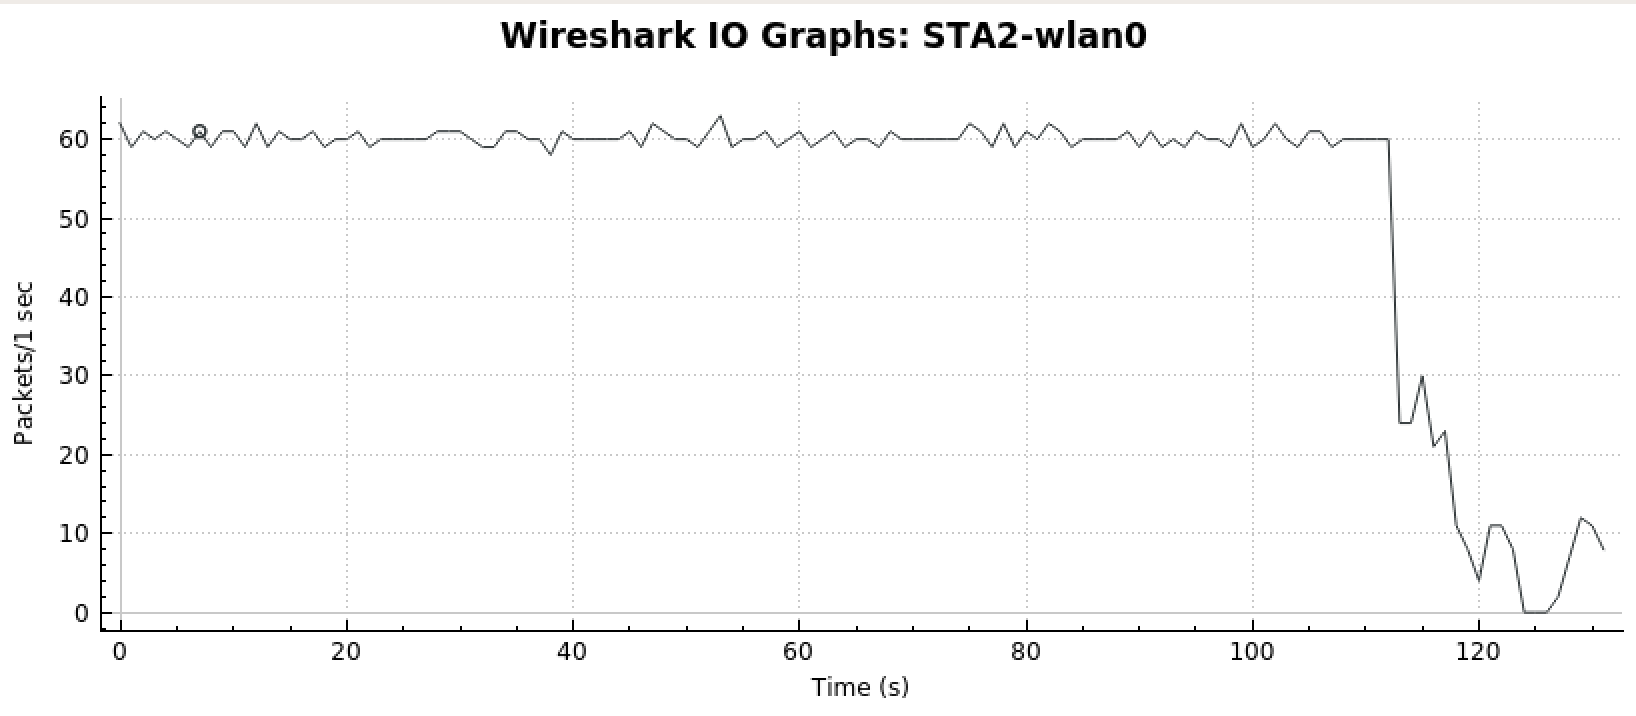
\includegraphics[width=0.6\linewidth]{batmand.png}
        		\caption{SIP connection \& throughput under BATMAND protocol}
        		\label{fig:t2-3}
    	\end{figure}
\par The figures 10, 11 \& 12 show the statistics from the SIP connection which lasts for 120 seconds on both server and client terminal CLI and the throughput graph from Wireshark. \\\\ Under the 'batman\_adv' protocol, the connection statistics on the server(STA1) shows;
	\begin{itemize}
		\item Cumulative Call Rate of 9.613 calls per second
		\item 1192 Successful Calls created
		\item 0 Failed Calls
	\end{itemize}
Under the 'batmand' protocol, the connection statistics on the server(STA1) shows;
	\begin{itemize}
		\item Cumulative Call Rate of 9.497 calls per second
		\item 1177 Successful Calls created
		\item 0 Failed Calls
	\end{itemize}
Under the 'olsrd' protocol, the connection statistics on the server(STA1) shows;
	\begin{itemize}
		\item Cumulative Call Rate of 9.531 calls per second
		\item 1182 Successful Calls created
		\item 0 Failed Calls
	\end{itemize}
\newpage
    	\begin{figure}[]
        		\centering
        		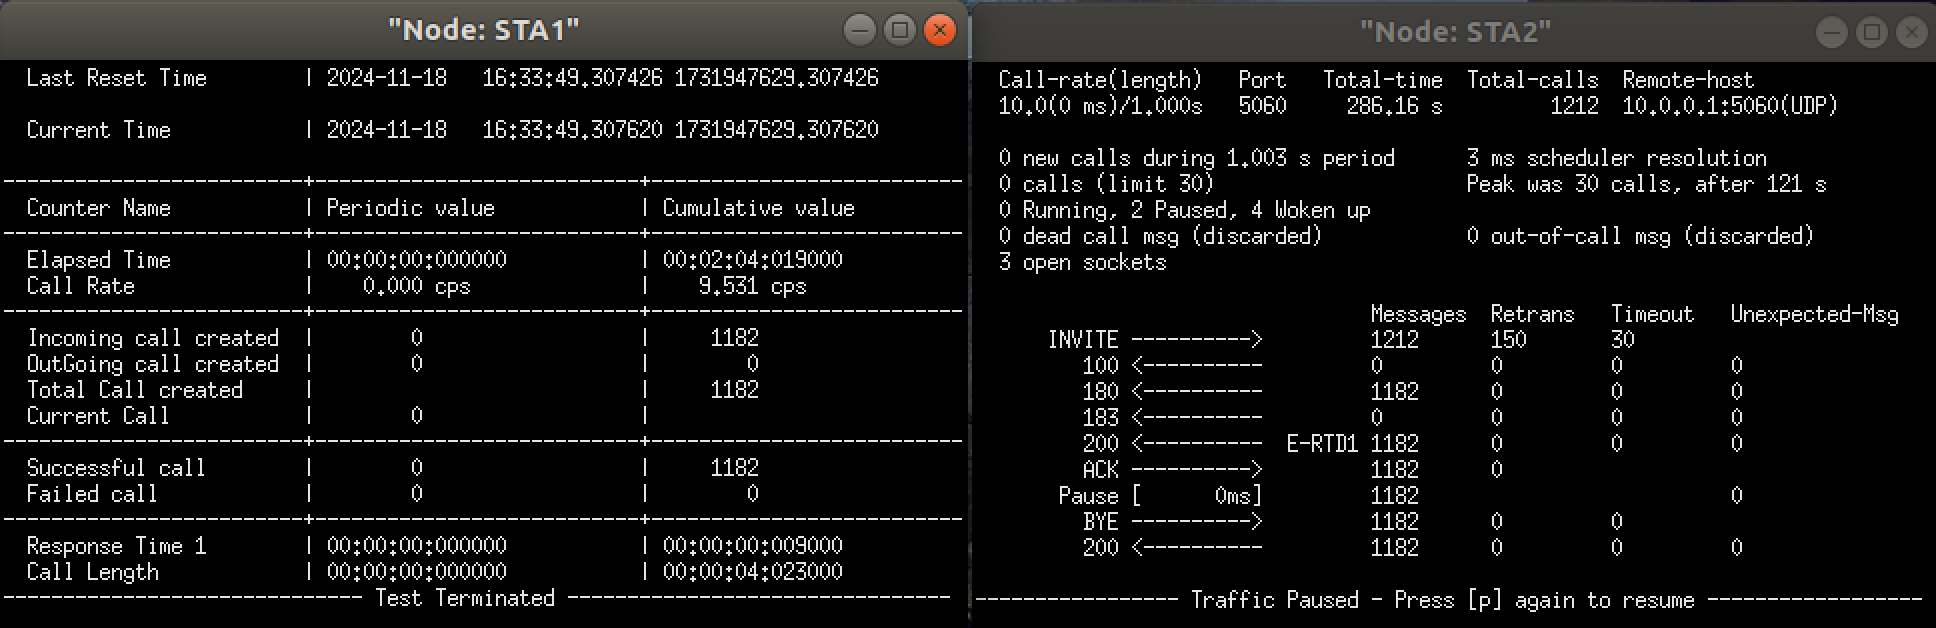
\includegraphics[width=0.6\linewidth]{olsrd1.png}
        		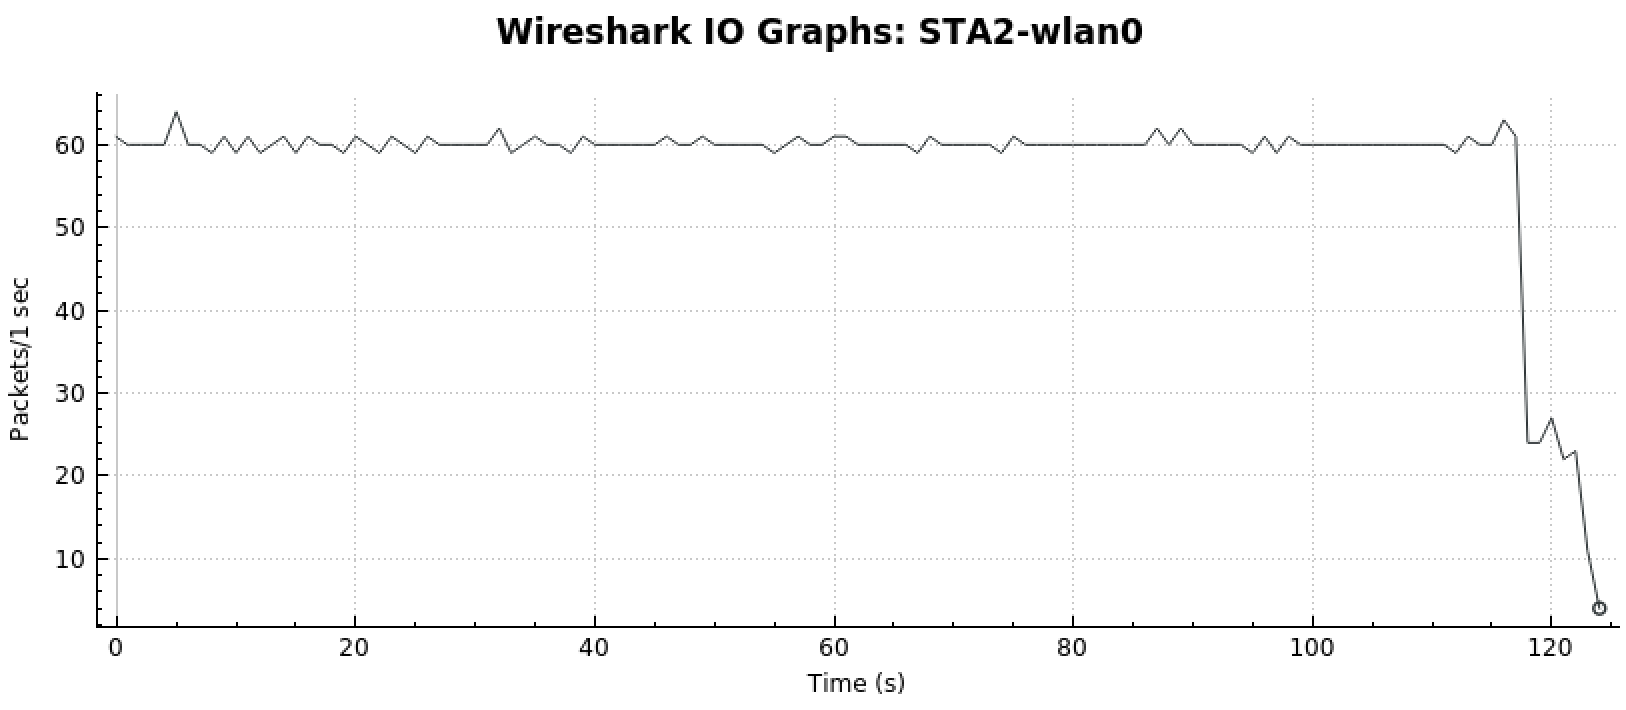
\includegraphics[width=0.6\linewidth]{olsrd.png}
        		\caption{SIP connection \& throughput under OLSRD protocol}
        		\label{fig:t2-4}
    	\end{figure}
\par At the end of this experiment, we have achieved a functioning adhoc network with successful VoIP connectivity under different adhoc protocols. Analysing the results from the statistics shows the best protocol to be the 'batman\_adv' protocol since it achieved the highest call rate however, we notice slight difference among the 3 protocols tested in terms of network performance, connections maintained, and average bandwidth maintained during transmission period.

\newpage
\section{Task 3 - SDN Simulation}
This task activity utilises the concept of Software Defined Networking in conjunction with OpenFlow on the local machine to manage our network. The experiment entails creating a network that connects an old building to a new building at the University of Hertfordshire. The task emulates 3 servers housed in the old building and 2 hosts in the new building. We utilise 5 switches for the underlying data forwarding and an SDN controller for the purpose of this activity. We also undertake a User Datagram Protocol(UDP) transmission  between two nodes for a specified duration, port number, and bandwidth. \\ A UDP transmission is a type of communication protocol which unlike Transmission Control Protocol(TCP)\cite{CONRAD201263} the communication does not require the three-way handshake(SYN - SYN\_ACK - ACK) to establish a secure connection.
	\begin{itemize}
		\item SYN - sender sends synchronisation message to receiver
		\item SYN\_ACK - receiver sends synchronisation-acknowledgement message to sender
		\item ACK - sender sends acknowledgment message to receiver to establish communication
	\end{itemize}  
The sender sends out packets without waiting for an acknowledgement from the recipient. This form of communication does check errors and may encounter loss of packets during transmission but in turn achieves higher transmission speeds and supports transfer of large size data.
\subsection{ONOS Controller}
ONOS stands for Open Network Operating System. ONOS provides the control plane for a software-defined network (SDN), managing network components, such as switches and links, and running software programs or modules to provide communication services to end hosts and neighbouring networks. It was developed by the ONOS Project, which is led by a collaboration of various universities and industry partners, including Intel and Ericsson. ONOS controller helps to attain the advantages of SDN by achieving network programmability, high-performance and scalability, support for OpenFlow protocols, support virtualisation of networks, fault tolerant and high-availability, and support for heterogeneity of network devices.
\subsection{Design and Configuration}
Table 4 contains the configuration information for hosts and servers in the network which is used in the python script for the network configuration. After completing the python script, the ONOS controller is built and started on a Linux terminal with the commands \texttt{bazel build onos} and \texttt{runsdn}. When the ONOS server is ready, we log in with \texttt{onos localhost} command from a new terminal where we have access to the controller and can activate some networking applications for the network to operate how we desire. The commands;
	\begin{itemize}
		\centering
		\item \texttt{app activate org.onosproject.openflow}
		\item \texttt{app activate org.onosproject.fwd}
	\end{itemize}
are used to activate flows and reactive routing on the controller which is necessary for transfer of packets across the network. Now, on a new terminal we run the network configuration file with the command; \\ \texttt{sudo mn --custom <python filename> --controller remote,ip=<ONOS controller IP> --topo <topo name>} which specifies the controller to be used for the network. \\ We access the ONOS GUI at \texttt{http://localhost:8181/onos/ui} to view the topology of the network which is shown in fig. 13. This is available only after all nodes can have full connectivity to each other, thus servers and hosts can communicate successfully. The hosts are made visible on the ONOS GUI by pressing the "H" key on the keyboard.
    	\begin{table}[h]
        		\centering
        		\begin{tabular}{|c|c|c|}
            		\hline
            		NAME & IPv4 & MAC ADDRESS \\
            		\hline
            		H1 & 192.170.50.11 & 00:00:00:00:15:98 \\
           		H2 & 192.170.50.12 & 00:00:00:00:15:99 \\
            		SERVER1 & 20.0.0.2 & 00:00:00:00:16:00 \\
            		SERVER2 & 40.0.0.2 & 00:00:00:00:16:01 \\
            		SERVER3 & 60.0.0.2 & 00:00:00:00:16:02 \\
            		\hline
        		\end{tabular}
        		\caption{Network configuration details}
        		\label{tab:4}
    	\end{table}
    	\begin{figure}[h]
        		\centering
        		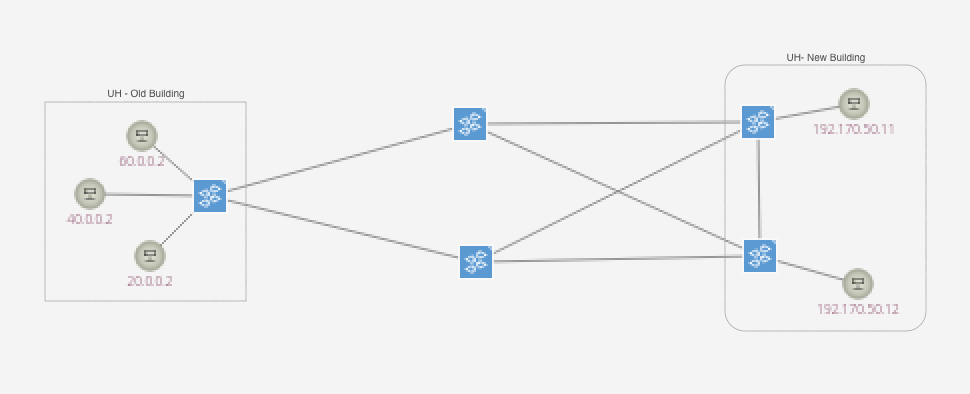
\includegraphics[width=0.8\linewidth]{t3-topo.png}
        		\caption{Network topology from ONOS GUI}
        		\label{fig:t3-1}
    	\end{figure}

\par As seen in the configuration details in Table 4, the hosts and servers are in different networks. Without any routing configured on the nodes, nodes will not be able to communicate with nodes in a different network. To solve this issue, we configured static routes on each node with information of the other network. The command below is a generic one of the routing configured on each node; 
	\begin{itemize}
		\centering
		\item \texttt{ip route add <network address>/<netmask>  dev <interface>}
	\end{itemize}
This can be carried out on the Mininet CLI, the ip route command preceded with the node name or directly on the node terminal CLI accessed with 'xterm' from Mininet. Once the route configurations are done, we can expect to have full connectivity in the network and proceed to the UDP transmission. To carry out this activity, a terminal CLI for both nodes(Server \& Host1) is launched using the 'xterm' command on Mininet. The 'iperf' is a command which can be used to stress-test a network to determine communication performance of the network. \\ On the server, we enter the command; 
	\begin{itemize}
		\item \texttt{iperf -s -u -p <port> -i 1} : initiate the server to listen for UDP connections on port specified for every second
	\end{itemize}
And on client, we enter command;
	\begin{itemize}
		\item \texttt{iperf -c <server IP> -u -p <port> -t <time> -b <bandwidth>} : start the UDP connection by the client to the server, at port, duration, and bandwidth specified
	\end{itemize}

\subsection{Results and Analysis}
After we activate the network apps on the ONOS controller and start the network on Mininet, we check the connectivity of nodes in our network prior to configuring static routes on each node. The fig. 14 has images of the results from a 'pingall' command in Mininet. \\ 
  	\begin{figure}[h]
		\minipage{0.5\textwidth}
			\centering
			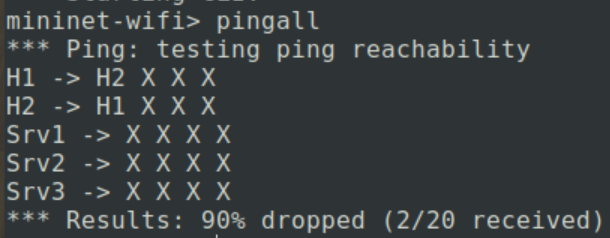
\includegraphics[width=0.7\linewidth]{t3-noping.png}
		\endminipage{} 
		\minipage{0.5\textwidth}
			\centering
			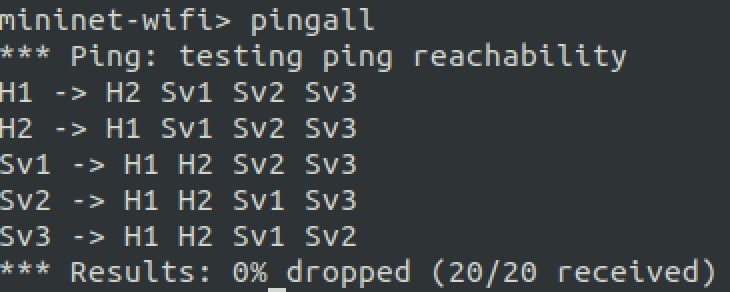
\includegraphics[width=0.7\linewidth]{t3-pingall.png}
		\endminipage{}
            	\caption{Connectivity tests before \& after reactive routing activation}
            	\label{fig:t3-2}
        \end{figure} 
\par As shown, 90\% of packets dropped from testing connectivity prior configuring the ip routes on nodes due to the nodes having no idea how to reach other networks outside their original network. Once the nodes have routing information to reach other networks, full connectivity is achieved as shown from 0\% packets dropped. \\\\  Then commenced the UDP communication between Server1 \& Host1 for 600 seconds, with bandwidth of 100 megabytes per second, and on port 5656 after full connectivity of the network is established. \\ The results from the UDP test in fig. 15 showed successful connection between Server1 \& Host1 with the following statistics;
	\begin{itemize}
		\item connection time of 600 seconds
		\item total jitter(time interval of packet arrival) of 0.161 milliseconds
		\item transferred total of 7.32 gigabytes of data
		\item maintained bandwidth of 105 megabytes per second
		\item 5349875 total datagrams sent and 250 datagrams received out-of-order
	\end{itemize}
        \begin{figure}[h]
        		\centering
		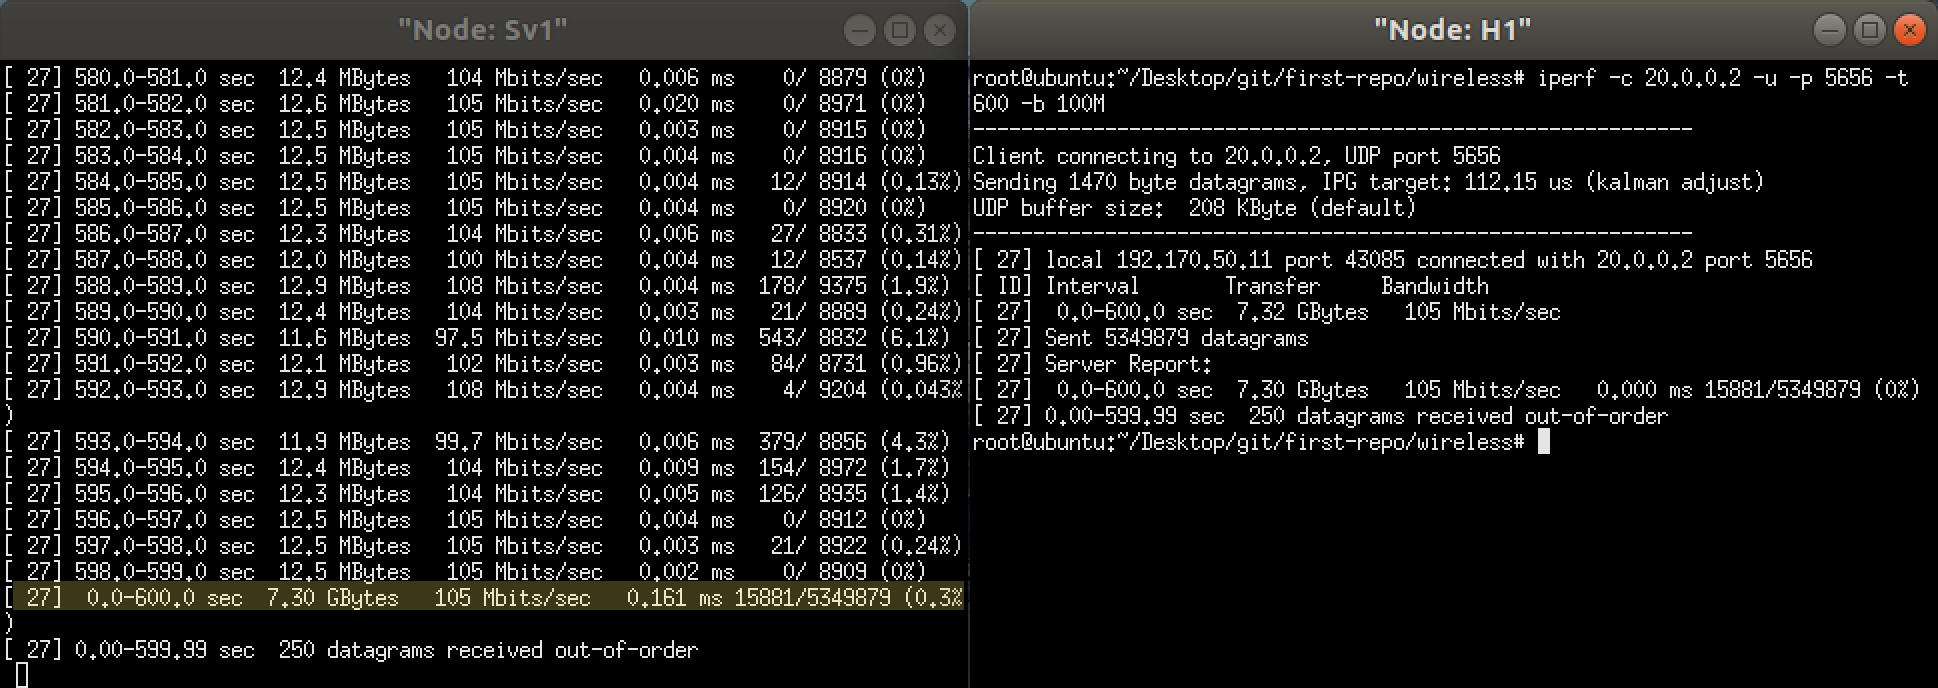
\includegraphics[width=1\linewidth]{t3-udp.png}
		\caption{UDP connection between Server \& Client}
		\label{fig:t3-3}
        \end{figure}
        
\newpage
\par In general, UDP based communications are faster compared to TCP based connections. This is due to the lack of error checks and the acknowledgement technique used by TCP to establish secure and less error in communications. \\
	\begin{figure}[h]
		\centering
		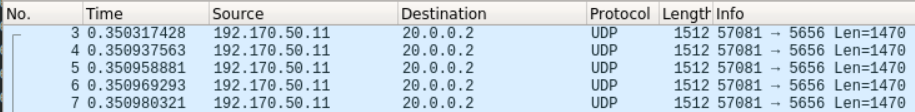
\includegraphics[width=1\linewidth]{t3-wireshark.png}
		\caption{Wireshark capture on H1-eth0 interface}
		\label{fig:t3-4}
	\end{figure}
\par This snippet from Wireshark gives details on how the UDP protocol works. The transfer is one-way(from Host1 to Server1) with no acknowledgment from Server1. This allows for high rate data transfer and beneficial in applications where data transfer is needed in real-time. \\ SDN supports the building and testing of such network scenarios with no reliant on infrastructure or hardware equipments, reduce expenses, and provides faster and convenient control of the entire network.

\newpage
\section{Task 4 - Multicast Video Stream Service}
The final experiment emulates a local area network(LAN) where we test the multicast video streaming over the network for the new building to facilitate learning. Multicasting\cite{0202020} in networking is a type of communication which is also known as a one-to-many communication. In a connectionless network, multicast basically involves replicating packets and distributing them to multiple receivers. A multicast group refers to a set of senders and receivers who are involved in a multi-party communication session. It is always advantageous to use multicast rather than multiple unicast communication since it provides efficient means of communication among selected nodes within a large network\cite{1010101}.
\subsection{Design and Configuration}
The network to be tested consist of 2 switches, a video source acting as server, and three host devices which could be any ethernet enabled device. Table 5 contains the name and IP address for configuration on host devices. The host devices will have the same network address and the configuration to allow for multicast communication is activated on video source(VS), host1(H1), and host2(H2) which creates a multicast group for these devices.
    	\begin{table}[h]
        		\centering
        		\begin{tabular}{|c|c|}
            		\hline
            		DEVICE NAME & IP ADDRESS \\
            		\hline
            		H1 & 50.10.10.10 \\
            		H2 & 50.10.10.11 \\
            		H3 & 50.10.10.12 \\
            		VS & 50.10.10.20 \\
            		\hline
        		\end{tabular}
        		\caption{Network configuration details}
        		\label{tab:5}
    	\end{table}
    	\begin{figure}[h]
        		\centering
        		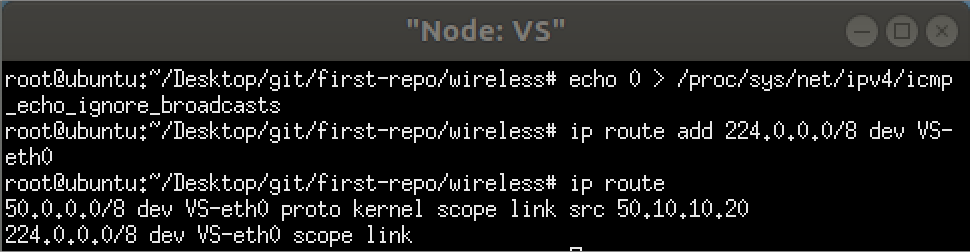
\includegraphics[width=0.7\linewidth]{mc-vs.png}
        		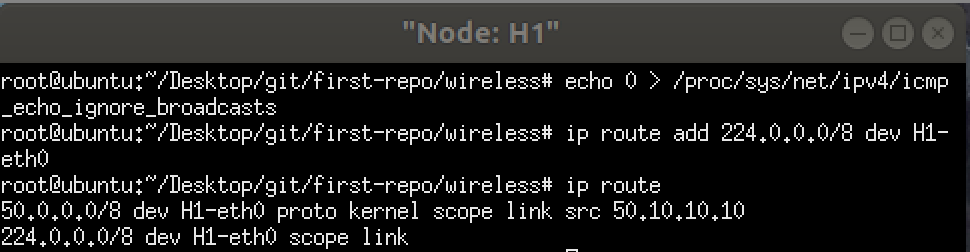
\includegraphics[width=0.7\linewidth]{mc-h1.png}
        		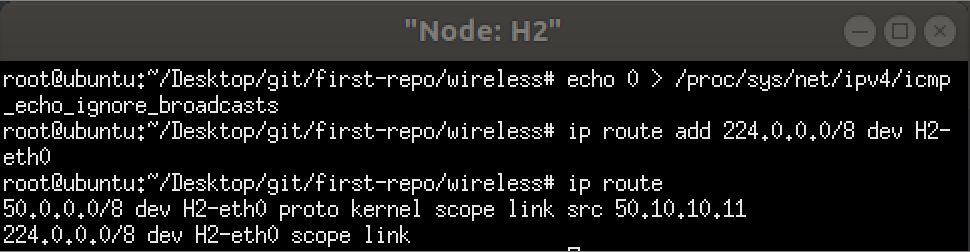
\includegraphics[width=0.7\linewidth]{mc-h2.png}
        		\caption{Activating multicast for required nodes}
        		\label{fig:t4-1}
    	\end{figure}

\newpage
Fig. 16 shows the steps in activating the multicast on the required nodes. This can be done directly on the Mininet or at the node terminal when accessed with 'xterm' command on Mininet. The commands;
	\begin{itemize}
		\item \texttt{echo 0 > /proc/sys/net/ipv4/icmp\_ignore\_broadcasts}: allow node response to Internet Control Message Protocol(ICMP) echo request(ping request) broadcasted to every host on the network
		\item \texttt{ip route add 224.0.0.0/8 dev <interface>}: configures route that ensures multicast traffic for 224.0.0.0/8 address range is sent through the interface specified
	\end{itemize}
    	\begin{figure}[h]
		\centering
        		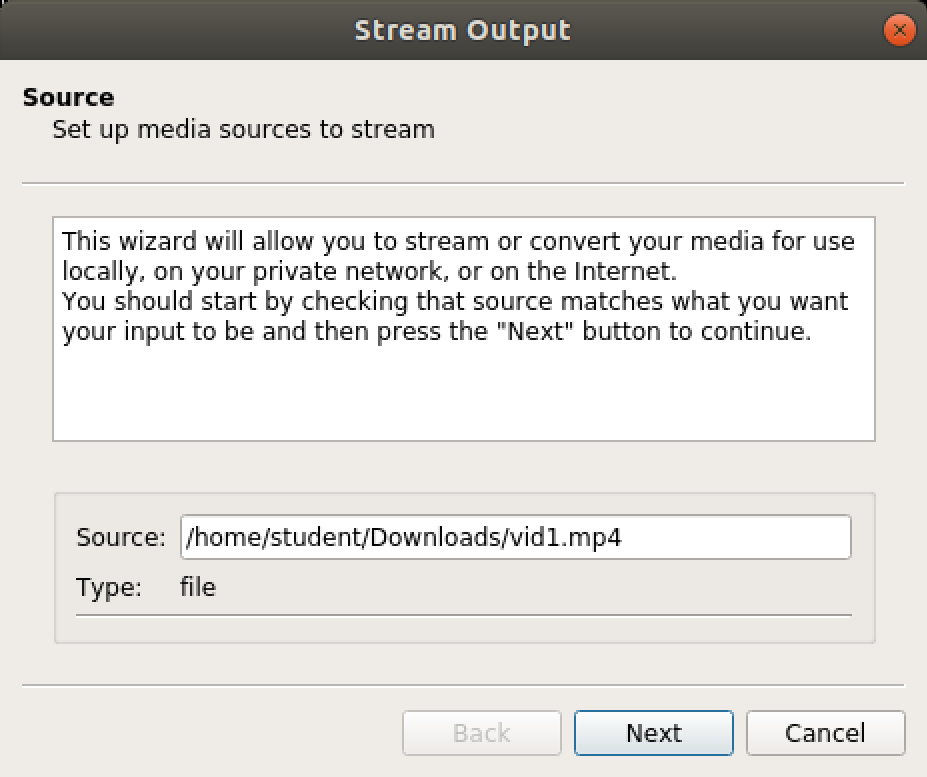
\includegraphics[width=0.35\linewidth]{vs-1.png}
        		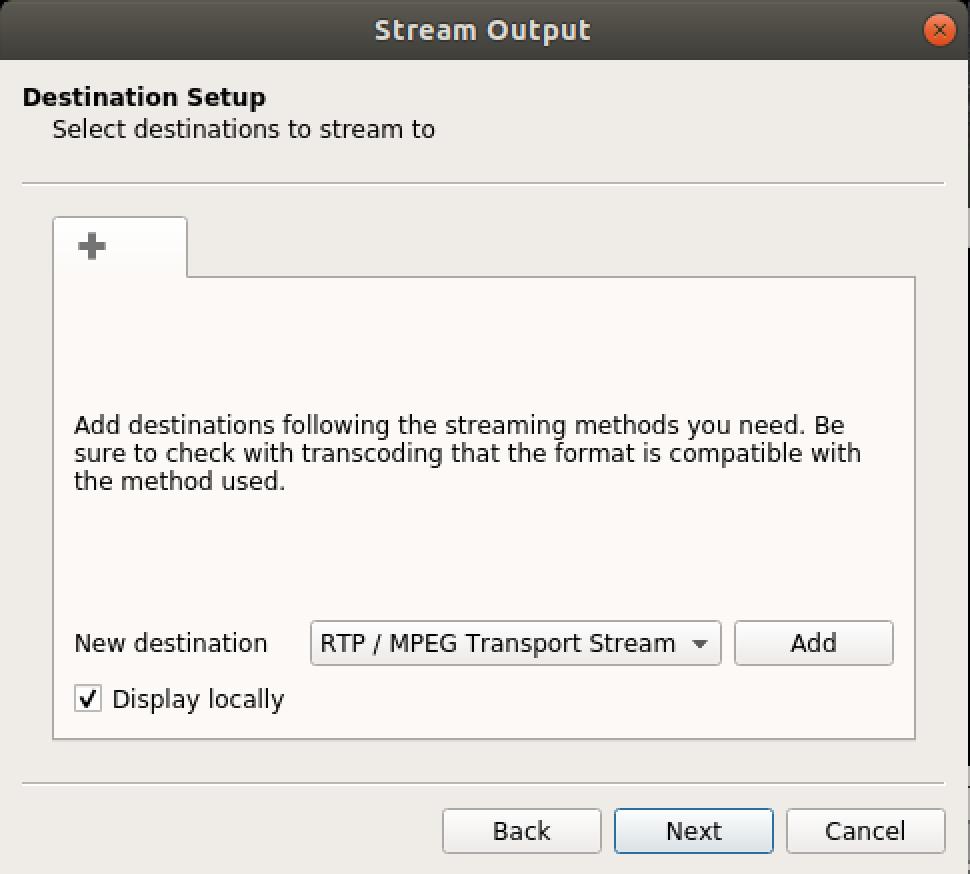
\includegraphics[width=0.35\linewidth]{vs-2.png}
        		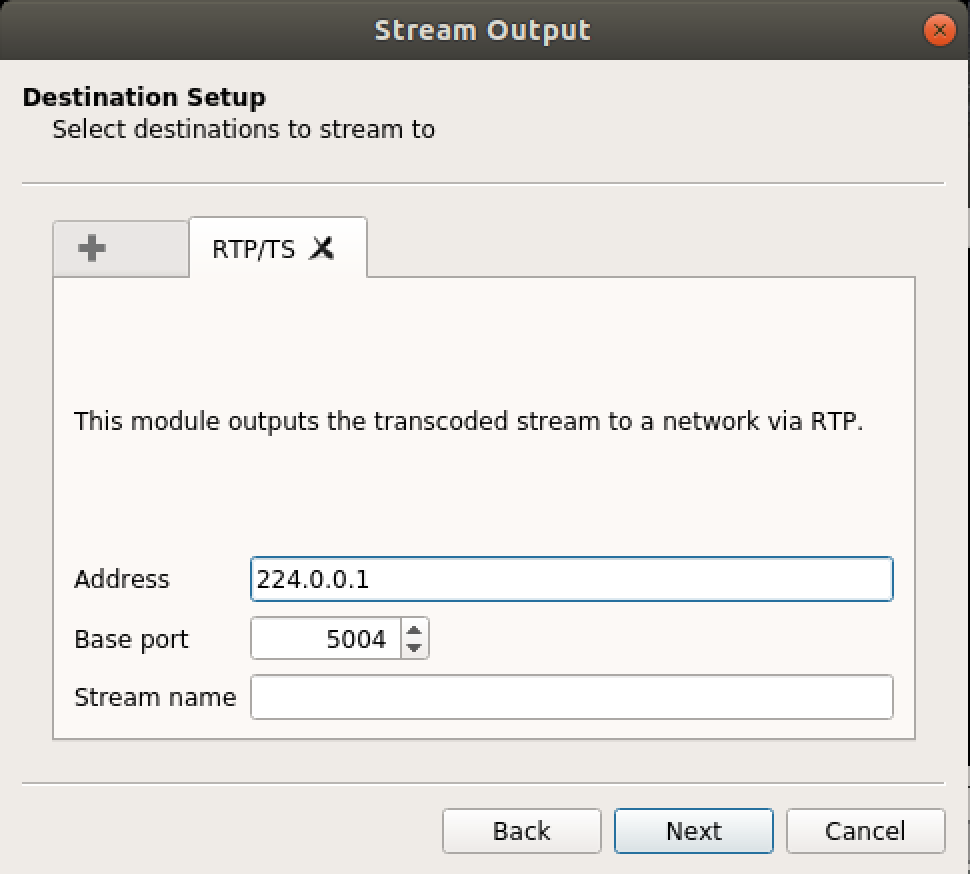
\includegraphics[width=0.35\linewidth]{vs-3.png}
        		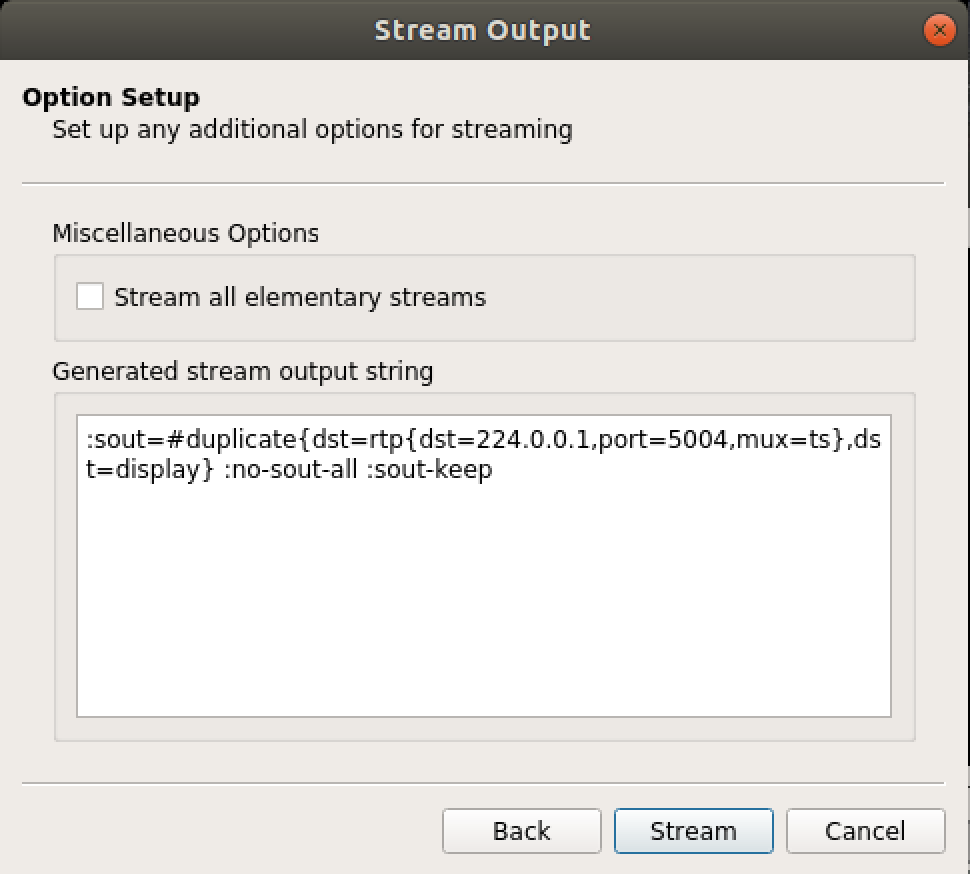
\includegraphics[width=0.35\linewidth]{vs-4.png}
        		\caption{Multicast streaming setup at video source}
        		\label{fig:t4-2}
    	\end{figure}
	\begin{figure}[h]
		\centering
		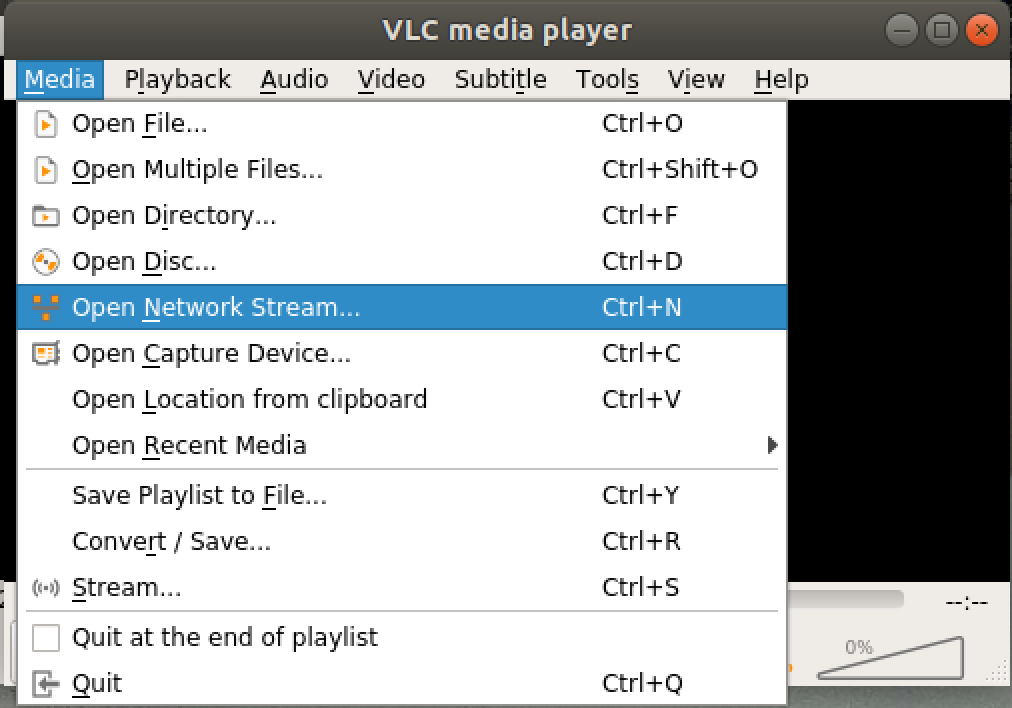
\includegraphics[width=0.35\linewidth]{t4-multcasthost1.png}
		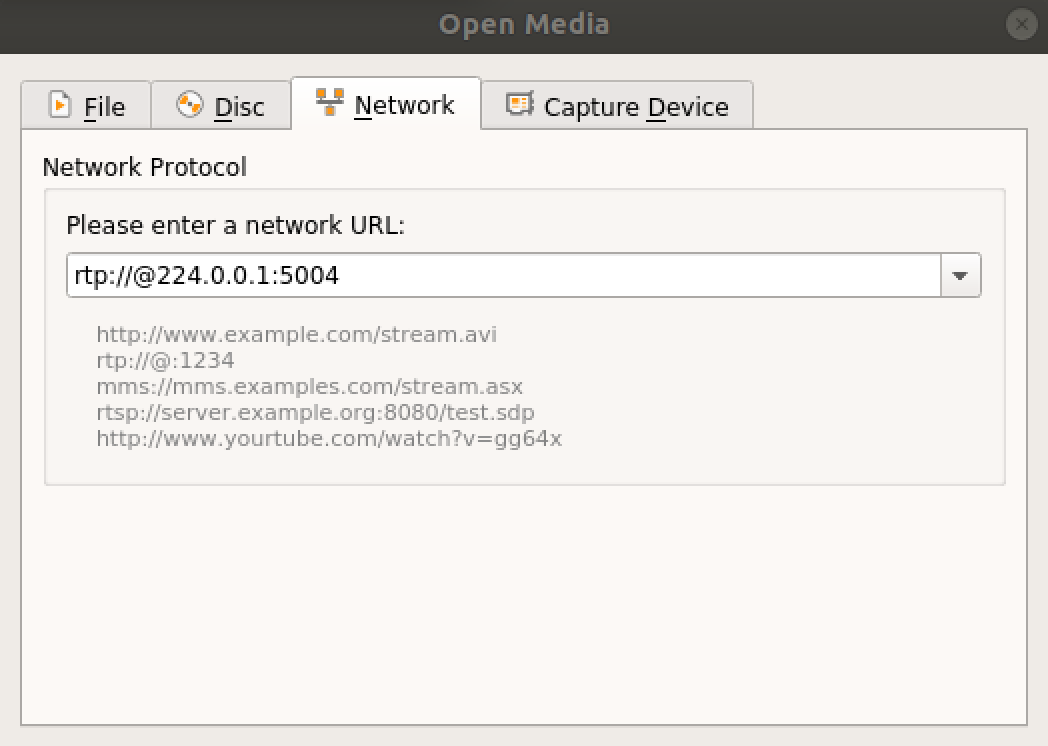
\includegraphics[width=0.35\linewidth]{t4-multcasthost.png}
		\caption{Multicast video connection at multicast host}
		\label{fig:t4-3}
	\end{figure}
After routing configuration, the video stream output is initiated from the video source on VLC through the terminal CLI of the video source, the command \texttt{vlc-wrapper} launches VLC where we select the video file, transfer protocol, and provide the network to which the streaming will be sent across. On the hosts terminal CLI, VLC is launched with the same command and the multicast video stream is connected using the URL \texttt{rtp://@224.0.0.1:5004}. Fig. 17 and 18 show these steps taken out respectively.

\subsection{Results and Analysis}
Once all configurations are completed, the video is seen on fig. 20 been streamed from the source across the multicast network where the two hosts(1 \& 2) can have the video output on the VLC player.
	\begin{figure}[h]
		\centering
		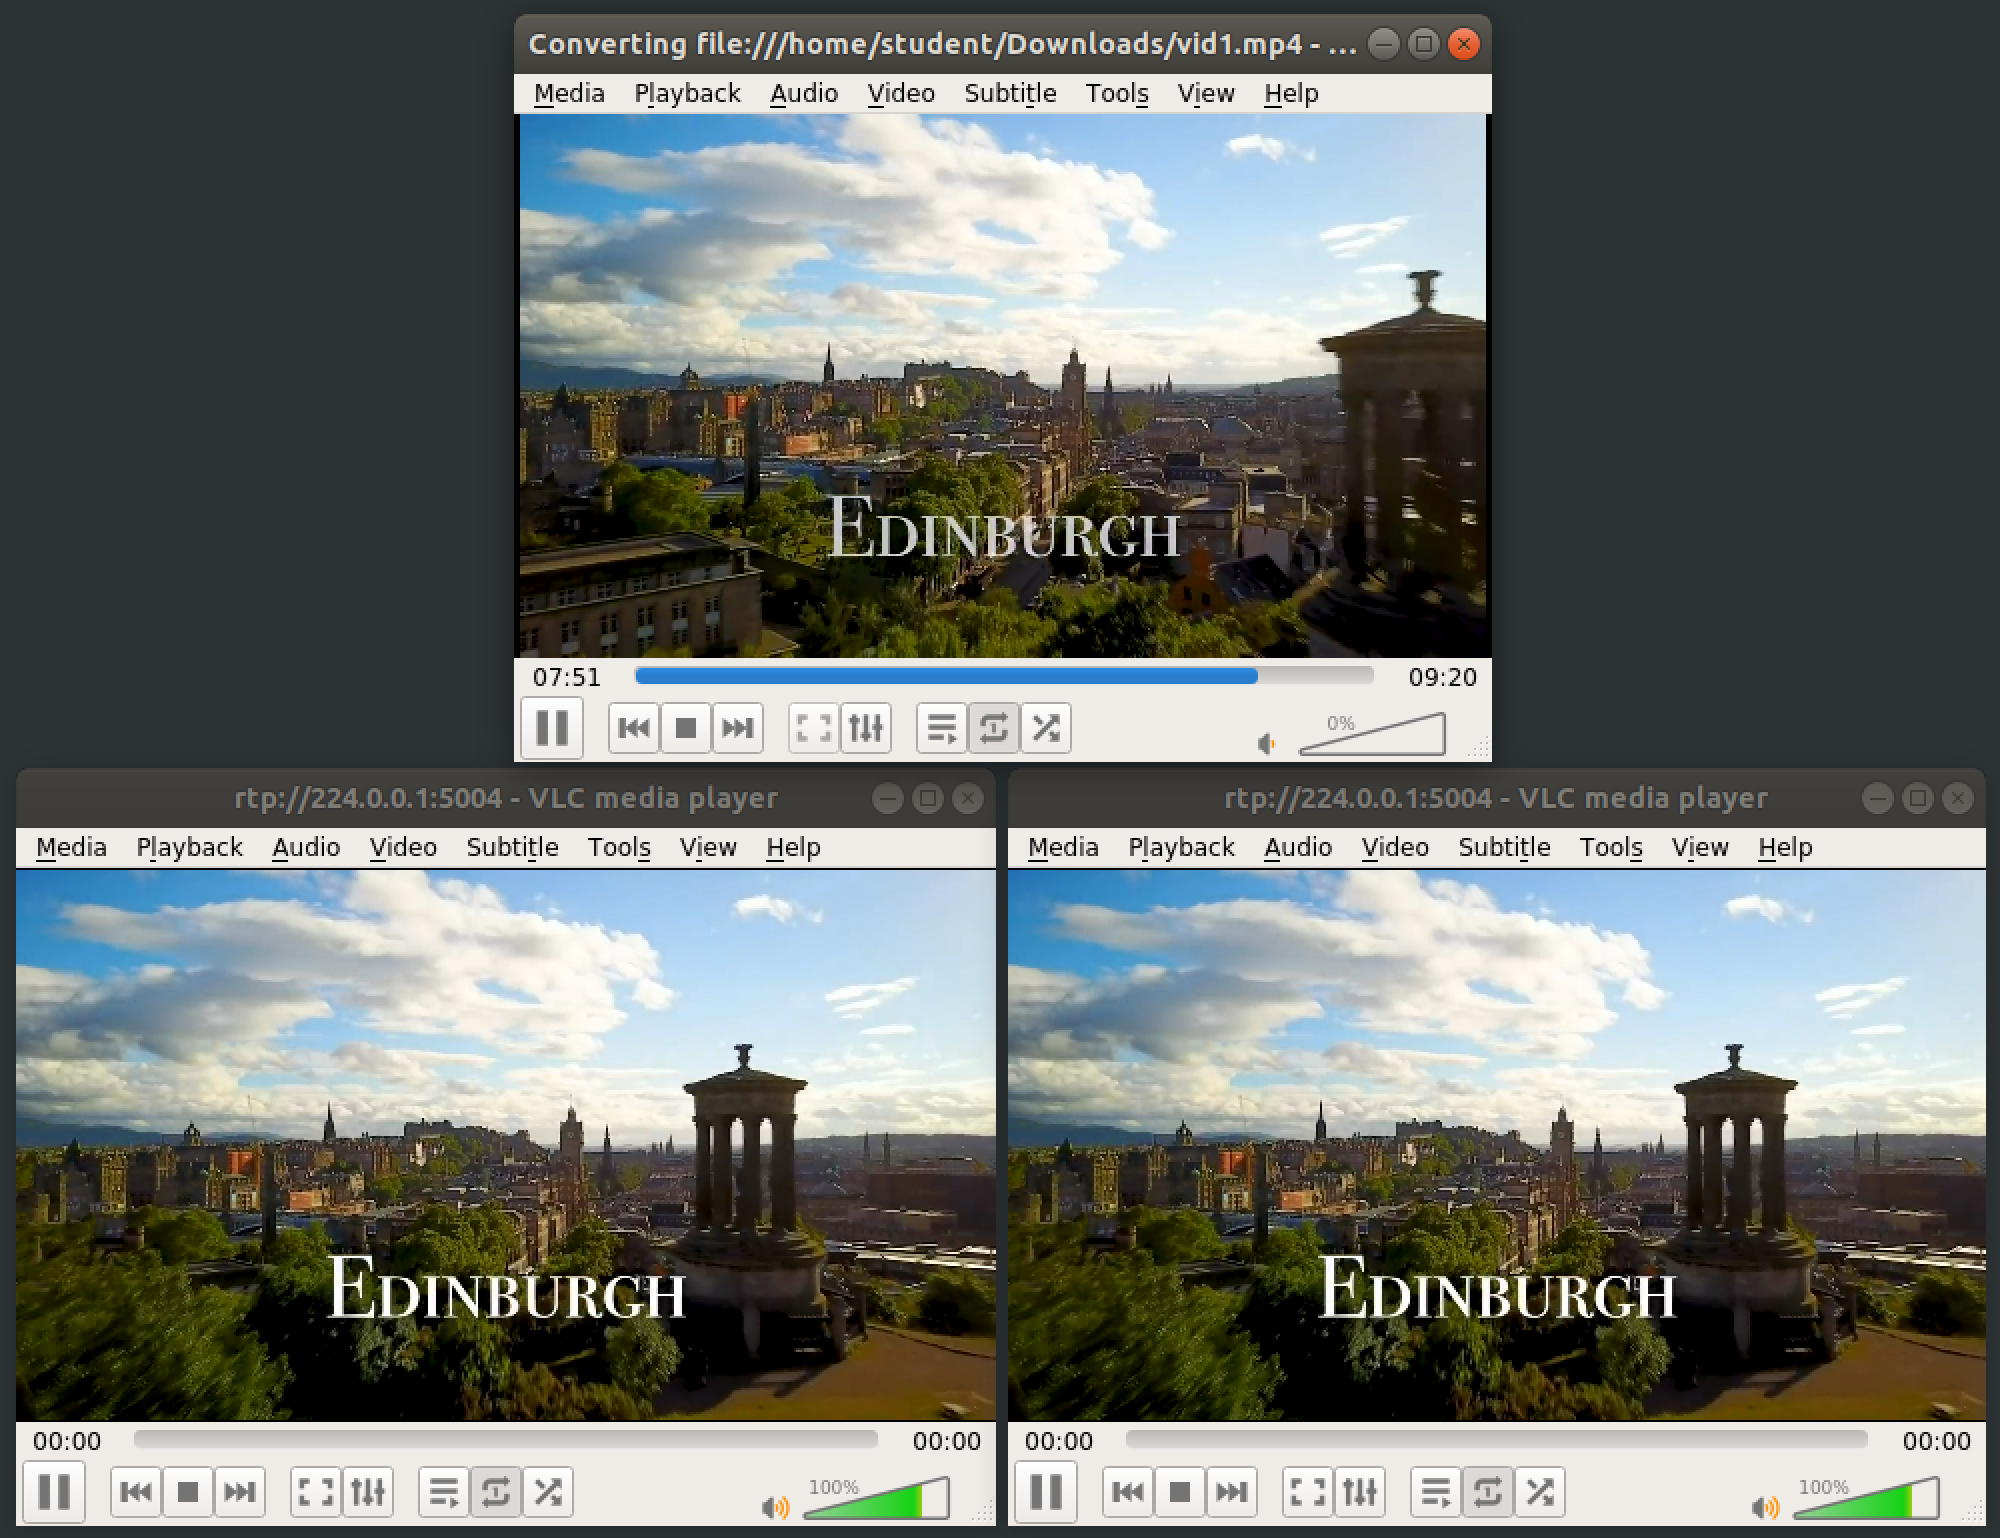
\includegraphics[width=0.5\linewidth]{t4-multcast.png}
		\caption{Multicast video stream from source to hosts}
		\label{fig:t4-4}
	\end{figure}
	\begin{figure}[h]
		\centering
		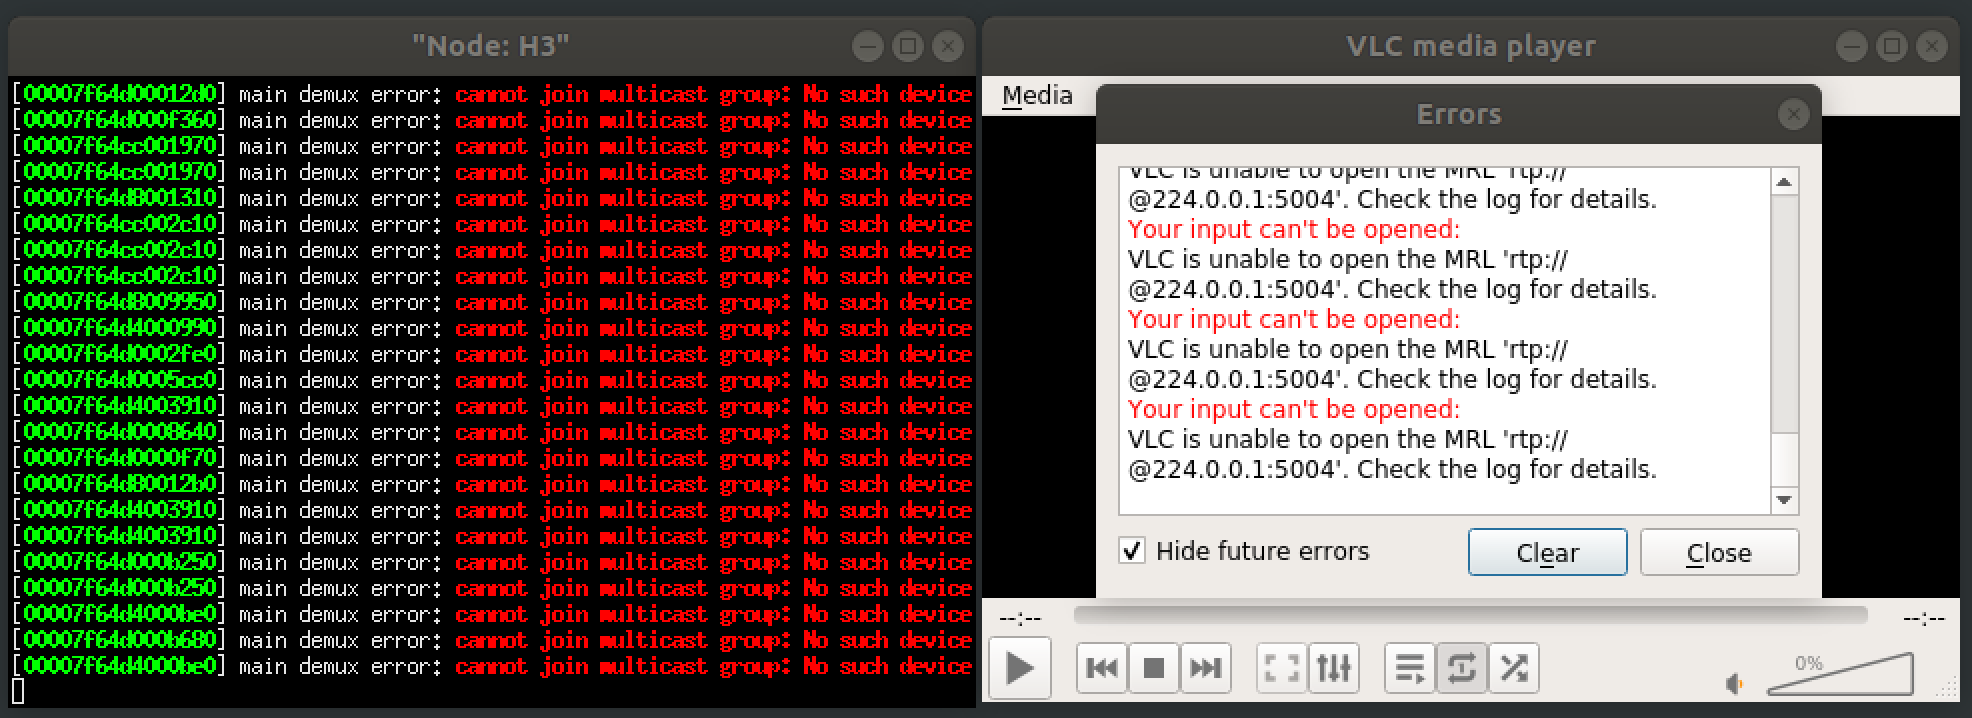
\includegraphics[width=0.7\linewidth]{t4-host3.png}
		\caption{Multicast video stream at host 3}
		\label{fig:t4-5}
	\end{figure}
\par The third host who is not part of the multicast group cannot stream the video as shown on fig. 21. This confirms that the streaming is a multicast stream and only host devices within the multicast group can get access to the video stream. Fig. 22 shows a snippet of a Wireshark capture where we can see from Ethernet section of the packet that the destination MAC address is of a multicast type(IPv4mcast\_01). \\\\ During this process, we encounter a protocol known as the Real-Time Transfer Protocol(RTP) which is a used for transmission of media files(audio or graphics) over an IP network. Since it is also a form of UDP connection so it does not require acknowledgment in setting up the communication which makes it able to support voice and video communications over IP and online gaming.

\newpage
	\begin{figure}[h]
		\centering
		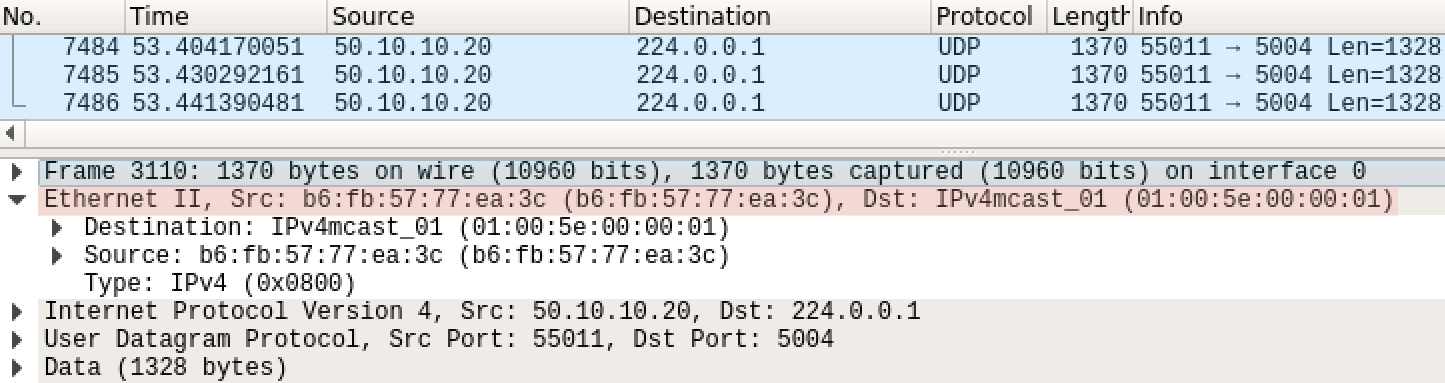
\includegraphics[width=0.9\linewidth]{t4-wireshark}
		\caption{Packet details captured on Wireshark}
		\label{fig:t4-6}
	\end{figure}
	
\section{Conclusion}
At the end of the experiments, it is confirmed that SDN provides greater advantages to network developers or operators in the manner of network control and also a summary of the network compared to the traditional way of computer networking. There are also vast improvements in the deployment of networks, configuration, fault tolerance, and scalability as demonstrated in the tasks. \\ The table below shows a comparison of some features between traditional and software-defined networking.
	\begin{table}[h]
		\small
		\centering
		\begin{tabular}{|c|c|c|}
			\hline
			Feature & Traditional Networking & Software-Defined Networking \\
			\hline
			Control plane & Distributed across devices & Centralised \& managed by SDN controller \\
			Network Configuration & Manual configuration & Configuration via software and APIs \\
			Agility \& Flexibility & Difficult to adapt quickly & Quick reconfiguration \\
			Cost Efficiency & High cost of infrastructure & Low cost due to virtualisation \\
			Programmability & Difficult to program & Easy to program via SDN controller \\
			\hline
		\end{tabular}
	\end{table}
\par To conclude, we point out the achievements of software-defined networking in the emulation of the wireless and ad-hoc network, in testing the Voice over IP(VoIP) communication, and the multicast streaming service over a network. The configuration and deployment of the networks required less time and effort, very low cost, and can be easily managed due to the agility and flexibility offered. Researchers and network designers can test out new ideas and innovations while network concepts can be taught in education setting in a very efficient and convenient way.

\newpage
\section{References}
\bibliographystyle{plain}
\bibliography{references}

\newpage
\section{Appendix}
\renewcommand{\thesection}{\alph{section}}
\setcounter{section}{0}
\section{Task 1 code}
\begin{lstlisting}
import sys
from mininet.node import Controller
from mininet.log import setLogLevel, info
from mn_wifi.cli import CLI
from mn_wifi.net import Mininet_wifi

def topology():
    info("**creating network**\n")
    net = Mininet_wifi()

    info("**creating nodes**\n")
    ap1 = net.addAccessPoint('ap1', mac='00:00:00:00:00:00', ssid='AP1', mode='g', channel='1', position='30,117.5', band='5', range=35)
    ap2 = net.addAccessPoint('ap2', mac='00:00:00:00:00:01', ssid='AP2', mode='g', channel='1', position='60,117.5', band='5', range=35)
    ap3 = net.addAccessPoint('ap3', mac='00:00:00:00:00:02', ssid='AP3', mode='g', channel='1', position='80,117.5', band='5', range=35)
    ap4 = net.addAccessPoint('ap4', mac='00:00:00:00:00:03', ssid='AP4', mode='g', channel='1', position='135,55', band='5', range=50)
    ap5 = net.addAccessPoint('ap5', mac='00:00:00:00:00:04', ssid='AP5', mode='g', channel='1', position='135,40', band='5', range=50)
    sta1 = net.addStation('iphone5', mac='00:00:00:00:00:10', ip='192.168.50.11/24', position='15,115', range=20, min_v=1, max_v=5)
    sta2 = net.addStation('ipad', mac='00:00:00:00:00:11', ip='192.168.50.12/24', position='20,130', range=20, min_v=5, max_v=10)
    sta3 = net.addStation('macbook', mac='00:00:00:00:00:12', ip='192.168.50.13/24', position='140,10', range=20, min_v=2, max_v=7)
    c0 = net.addController('c0')
    net.setPropagationModel(model="logDistance", exp=5)

    info("**configuring wifi nodes and mobility**\n")
    net.configureWifiNodes()
    net.addLink(ap1, ap2)
    net.addLink(ap2, ap3)
    net.addLink(ap3, ap4)
    net.addLink(ap4, ap5)
    net.plotGraph(min_x=-20, min_y=-10, max_x=200, max_y=180)

    net.startMobility(time=0)
    net.mobility(sta1, 'start', time=10, position='15,115')
    net.mobility(sta1, 'stop', time=20, position='115,10')
    net.mobility(sta2, 'start', time=30, position='20,130')
    net.mobility(sta2, 'stop', time=60, position='150,10')
    net.mobility(sta3, 'start', time=25, position='140,10')
    net.mobility(sta3, 'stop', time=60, position='15,110')
    net.stopMobility(time=120)

    info("**starting network**\n")
    net.build()
    c0.start()
    ap1.start([c0])
    ap2.start([c0])
    ap3.start([c0])
    ap4.start([c0])
    ap5.start([c0])

    info("**running CLI**\n")
    CLI(net)

    info("**stopping network**\n")
    net.stop()

if __name__ == '__main__':
    setLogLevel('info')
    plot = False if '-p' in sys.argv else True
    topology()
\end{lstlisting}


\section{Task 2 code}
\begin{lstlisting}
import sys
from mininet.log import setLogLevel, info
from mn_wifi.link import wmediumd, adhoc
from mn_wifi.cli import CLI
from mn_wifi.net import Mininet_wifi
from mn_wifi.wmediumdConnector import interference

def topology(args):
    "Create a network"
    net = Mininet_wifi(link=wmediumd, wmediumd_mode=interference) 

    info("*** Creating nodes\n")
    sta1 = net.addStation('STA1', ip6='2024::11', mac='00:00:00:00:01:11', position='20,10,0', range=30, antennaGain=5, antennaHeight=1)
    sta2 = net.addStation('STA2', ip6='2024::12', mac='00:00:00:00:01:12', position='45,10,0', range=30, antennaGain=6, antennaHeight=2)
    sta3 = net.addStation('STA3', ip6='2024::13', mac='00:00:00:00:01:13', position='70,10,0', range=30, antennaGain=7, antennaHeight=3)
    net.setPropagationModel(model="logDistance", exp=4)

    info("*** Configuring nodes\n")
    net.configureNodes()

    info("*** Creating links\n")
    #testing 'batman_adv', 'batmand', 'olsrd' manet protocol
    net.plotGraph(min_x=-20, min_y=-40, max_x=120, max_y=90)
    net.addLink(sta1, cls=adhoc, intf='STA1-wlan0', ssid='adhocUH', mode='g', channel=5, ht_cap='HT40+', proto='batman_adv')
    net.addLink(sta2, cls=adhoc, intf='STA2-wlan0', ssid='adhocUH', mode='g', channel=5, ht_cap='HT40+', proto='batman_adv')
    net.addLink(sta3, cls=adhoc, intf='STA3-wlan0', ssid='adhocUH', mode='g', channel=5, ht_cap='HT40+', proto='batman_adv')
    
    info("*** Starting network\n")
    net.build()

    info("*** Running CLI\n")
    CLI(net)

    info("*** Stopping network\n")
    net.stop()

if __name__ == '__main__':
    setLogLevel('info')
    topology(sys.argv)
\end{lstlisting}

\section{Task 3 code}
\begin{lstlisting}
from mininet.topo import Topo  
from mininet.node import CPULimitedHost, Host, Node
from mininet.node import OVSSwitch
from mininet.topo import Topo

class MyTopo(Topo):  
	"Simple topology with VLAN support."
    	def __init__(self):
        	"Create custom topology."

	        # Initialize topology
	        Topo.__init__(self)

	        h1 = self.addHost( 'H1', mac='00:00:00:00:15:98', ip='192.170.50.11/24' )
	        h2 = self.addHost( 'H2', mac='00:00:00:00:15:99', ip='192.170.50.12/24' )
	        SERVER1 = self.addHost( 'Sv1', mac='00:00:00:00:16:00', ip='20.0.0.2/8' )
	        SERVER2 = self.addHost( 'Sv2', mac='00:00:00:00:16:01', ip='40.0.0.2/8' )
	        SERVER3 = self.addHost( 'Sv3', mac='00:00:00:00:16:02', ip='60.0.0.2/8' )

	        Switch1 = self.addSwitch( 'Switch1', cls=OVSSwitch )
	        Switch2 = self.addSwitch( 'Switch2', cls=OVSSwitch )
	        Switch3 = self.addSwitch( 'Switch3', cls=OVSSwitch )
	        Switch4 = self.addSwitch( 'Switch4', cls=OVSSwitch )
	        Switch5 = self.addSwitch( 'Switch5', cls=OVSSwitch )

	        self.addLink( h1, Switch4 )
	        self.addLink( h2, Switch5 )
	        self.addLink( SERVER1, Switch1 )
	        self.addLink( SERVER2, Switch1 )
	        self.addLink( SERVER3, Switch1 )
	        self.addLink( Switch1, Switch2 )
	        self.addLink( Switch1, Switch3 )
	        self.addLink( Switch2, Switch4 )
	        self.addLink( Switch2, Switch5 )
	        self.addLink( Switch3, Switch4 )
	        self.addLink( Switch3, Switch5 )
	        self.addLink( Switch4, Switch5 )

topos = { 'mytopo': ( lambda: MyTopo() ) }
\end{lstlisting}

\newpage
\section{Task 4 code}
\begin{lstlisting}
from mininet.topo import Topo
from mininet.net import Mininet
from mininet.node import Node
from mininet.log import setLogLevel, info
from mininet.cli import CLI

class MyTopo( Topo ):  
    "Simple topology example."
    def __init__( self ):
        "Create custom topo."

        # Initialize topology
        Topo.__init__( self )

        # hosts and switches 
        h1 = self.addHost('H1', ip='50.10.10.10/8')
        h2 = self.addHost('H2', ip='50.10.10.11/8')
        h3 = self.addHost('H3', ip='50.10.10.12/8')
        h4 = self.addHost('vidSrc', ip='50.10.10.20/8')
        s1 = self.addSwitch('s1')
        s2 = self.addSwitch('s2')

        self.addLink(h1, s2)
        self.addLink(h2, s2)
        self.addLink(h3, s2)
        self.addLink(s1, s2)
        self.addLink(h4, s1)

topos = { 'mytopo': ( lambda: MyTopo() ) } 
\end{lstlisting}
\end{document}
